%% 
%% Ultra-LSNT: Applied Energy Manuscript (Complete Merged Version)
%% 
\documentclass[review,3p,times]{elsarticle} 
% Remove 'draft' for final version

%% ==================== PACKAGES ====================
\usepackage{lineno,hyperref}
\usepackage{amsmath,amssymb,amsfonts}
\usepackage{multicol}
\usepackage{graphicx}
\graphicspath{{./}{figures/}{ablation/}}
\usepackage{booktabs}
\usepackage{multirow}
\usepackage{siunitx}
\usepackage{algorithm}
\usepackage{algorithmic}
\usepackage{color}
\usepackage{caption}
\usepackage{subcaption}
\usepackage{float}
\usepackage{enumitem}
\usepackage{xcolor}
\usepackage{threeparttable}
\usepackage{eurosym}
\setlength{\emergencystretch}{3em}
\modulolinenumbers[5]

\journal{Applied Energy}

%% ==================== FRONTMATTER EXTRAS ====================
% Applied Energy / Elsevier:
% - Highlights are REQUIRED and must be uploaded as a separate editable file.
% - Graphical Abstract is encouraged and must be uploaded as a separate file.
% You may keep placeholders in the manuscript for internal review.
% Set this switch to true if you want Highlights/Graphical Abstract to appear in the compiled PDF.
\newif\ifincludefrontmatterextras
\includefrontmatterextrasfalse

% Fallback stubs (in case a different class is used accidentally).
\makeatletter
\@ifundefined{highlights}{%
 \newenvironment{highlights}{\par\noindent\textbf{Highlights}\par\begin{itemize}\itemsep0pt}{\end{itemize}\par}%
}{}
\@ifundefined{graphicalabstract}{%
 \newenvironment{graphicalabstract}{\par\noindent\textbf{Graphical abstract}\par}{\par}%
}{}
\makeatother


\bibliographystyle{elsarticle-num}
\pdfstringdefDisableCommands{\def\corref#1{}}

\begin{document}

\begin{frontmatter}

%% ==================== TITLE ====================
\title{Unlocking the operational value of edge-based wind forecasting: a resilient sparse mixture-of-experts approach against SCADA imperfections}

%% ==================== AUTHORS ====================
\author[1]{Junyu Li}
\ead{ljylikezmn999@gmail.com}

\author[1]{Juntao Du\corref{cor1}}
\ead{dujuntao@aufe.edu.cn}
\cortext[cor1]{Corresponding author.}

\affiliation[1]{organization={School of Statistics and Applied Mathematics, Anhui University of Finance and Economics},
 city={Bengbu},
 postcode={233030},
 country={China}}

%% ==================== GRAPHICAL ABSTRACT ====================
% NOTE (submission): upload as a separate file via Editorial Manager.
\ifincludefrontmatterextras

% NOTE (submission): Graphical Abstract should be uploaded as a separate file.
\begin{graphicalabstract}
\centering
\IfFileExists{graphical_abstract.pdf}{%
 \includegraphics[width=\textwidth]{graphical_abstract.pdf}%
}{%
 \fbox{\parbox{0.96\textwidth}{\centering \textbf{Graphical abstract placeholder.}\\
 Replace with \texttt{graphical\_abstract.pdf} at submission (recommended 531$\times$1328 px, H$\times$W).}}%
}
\end{graphicalabstract}
\fi

%% ==================== HIGHLIGHTS ====================
% NOTE (submission): upload as a separate file via Editorial Manager.
\ifincludefrontmatterextras

% NOTE (submission): Elsevier requires Highlights to be uploaded as a separate editable file (3--5 bullets, each \leq 85 characters).
\begin{highlights}
\item Outperforms strong linear baselines under 60\% noise via sparse routing.
\item Cuts dispatch cost by 34\% and curtailment by 60\% under SCADA noise.
\item Reports latency, energy per inference, and model size for edge deployment.
\item Sparse expert routing supports interpretable and auditable operation.
\end{highlights}
\fi

%% ==================== ABSTRACT ====================
\begin{abstract}
Operational wind-farm SCADA streams are inherently noisy and drifting, and communication bandwidth is often limited.
This creates a deployment gap: models that appear competitive on curated benchmarks can degrade under sensing imperfections, leading to inflated reserve procurement and dispatch costs.
We propose Ultra-LSNT, a conditional sparse mixture-of-experts (MoE) forecaster for on-site edge inference under imperfect sensing and tight compute and memory budgets.
Edge deployment is motivated by latency reduction, resilience to intermittent connectivity, and local data governance because forecasts can be generated without exporting raw SCADA streams.
Evaluated on a real-world wind-farm SCADA dataset (Wind (CN), Xinjiang; publicly released) and GEFCom2012 under a unified inverse-scaling pipeline, Ultra-LSNT maintains predictive stability under severe perturbations.
Under additive noise up to 60\% of the clean-signal standard deviation, Ultra-LSNT retains $R^2>0.72$ on Wind (CN), whereas a strong linear baseline (DLinear) collapses.
In a 120-day rolling day-ahead dispatch backtest, Ultra-LSNT reduces total operating cost from 54.47M to 35.97M CNY ($\approx$34\%) and curtailment from 55.71M to 22.09M kWh (60\%) in a copper-plate setting.
In a complementary network-constrained DC-OPF study (IEEE RTS-24, $w_{\max}=260$ MW), curtailment reduction persists (12\%), confirming that the curtailment reduction persists even under explicit transmission constraints.
Ultra-LSNT also reduces feasibility-restoration (fallback) days from 75/120 (62.50\%) to 29/120 (24.17\%), serving as a numerical-solver stress indicator and a proxy for operational feasibility.
Finally, latency, model size, and energy per inference are reported as transparency metrics aligned with ``Green AI'', while the primary contribution is the quantification of robustness-driven operational value under realistic SCADA conditions. Finally, we argue that robustness stress tests under SCADA imperfections, together with transparent footprint reporting, should complement clean-benchmark accuracy in operational forecasting qualification.
\end{abstract}





%% ==================== KEYWORDS ====================
\begin{keyword}
Wind power forecasting \sep Economic dispatch \sep SCADA imperfections \sep Edge computing \sep Robustness \sep Wind power integration
\end{keyword}

\end{frontmatter}

\linenumbers

%% ==================== ABBREVIATIONS ====================
\section*{Abbreviations}
\noindent
\textbf{MoE}, Mixture-of-Experts;
\textbf{SCADA}, Supervisory Control and Data Acquisition;
\textbf{TSFM}, Time-series foundation model;
\textbf{LSTM}, Long Short-Term Memory;
\textbf{GRU}, Gated Recurrent Unit;
\textbf{GBDT}, Gradient Boosting Decision Tree;
\textbf{LightGBM}, Light Gradient Boosting Machine;
\textbf{FFN}, Feed-Forward Network;
\textbf{SOTA}, State-of-the-Art;
\textbf{MSE}, Mean Squared Error;
\textbf{MAE}, Mean Absolute Error;
\textbf{RMSE}, Root Mean Square Error;
\textbf{ABL}, Atmospheric Boundary Layer.

%% ==================== NOMENCLATURE ====================
\section*{Nomenclature}
\begin{center}
\fbox{%
\begin{minipage}{0.97\textwidth}
\small
\begin{multicols}{2}
\setlength{\tabcolsep}{4pt}
\renewcommand{\arraystretch}{1.15}
\begin{tabular}{@{}p{0.20\columnwidth}p{0.74\columnwidth}@{}}
\toprule
Symbol & Description \\
\midrule
$L$ & input length (time steps) \\
$H$ & prediction horizon (time steps) \\
$C$ & number of input variables/covariates \\
$\mathbf{X}\in\mathbb{R}^{L\times C}$ & input sequence \\
$\hat{\mathbf{Y}}\in\mathbb{R}^{H\times 1}$ & forecast output (wind power / target variable) \\
$\sigma_{\mathrm{cfg}}$ & configured perturbation ratio in robustness tests (dimensionless) \\
$\sigma_{\mathrm{eff}}$ & effective perturbation ratio, $\sigma_{\mathrm{eff}}=\alpha\sigma_{\mathrm{cfg}}$ \\
$\alpha$ & industrial scaling factor for injected noise ($\alpha=1.5$) \\
$K$ & number of selected experts in Top-$K$ routing \\
$\lambda$ & load-balancing regularization coefficient for routing \\
$\tau$ & Jump Gate threshold for conditional skipping \\
$R^2$ & coefficient of determination (scale-free) \\
RMSE/MAE & absolute errors in original physical units after inverse scaling \\
$E_{\text{inf}}$ & estimated energy per sample inference (mJ) \\
$B$ & batch size used in profiling (dimensionless) \\
$N_{\text{call}}$ & number of forecasting calls per day \\
$N_{\text{turb}}$ & number of turbines in a wind farm or fleet \\
$c_f$ & fuel / purchase price coefficient in dispatch (CNY/kWh) \\
$c_r$ & reserve price coefficient (CNY/kWh) \\
$c_s$ & storage discharge cost coefficient (CNY/kWh) \\
$c_{\text{su}}$ & start-up / shut-down cost coefficient (CNY) \\
$P_{\text{ch},\max}$ & storage charging power limit (kW) \\
$P_{\text{dis},\max}$ & storage discharging power limit (kW) \\
$S_{\max}$ & storage energy capacity limit (kWh) \\
$R_{\max}$ & thermal ramp-rate limit (kW per hour) \\
$\bar{P}_{\text{dev}}$ & average device power during inference (W) \\
\bottomrule
\end{tabular}
\end{multicols}
\end{minipage}}
\end{center}

\section{Introduction}
\label{sec:intro}

The increasing penetration of wind power raises the importance of reliable short-term forecasting for reserve scheduling and economic dispatch. In operational settings, forecast errors propagate to reserve procurement, curtailment decisions, and overall dispatch cost. Forecasting is typically based on Supervisory Control and Data Acquisition (SCADA) measurements collected at wind farms, where sensor noise, calibration drift, missing values, and quantization can occur. Many deployments also rely on resource-constrained edge hardware located close to the assets, which limits the applicability of compute-heavy models. This constraint is increasingly relevant as large pre-trained predictors are explored in energy forecasting \cite{gao2025mmgpt,wu2024stellm}. However, most time-series forecasting studies report accuracy under clean measurements and assume server-class deployment. This mismatch creates a deployment gap between benchmark performance and field requirements. A second gap is evaluative: peak clean-data accuracy does not necessarily imply robust behavior under realistic sensing imperfections or improved downstream decisions. On our Wind (CN) benchmark, a strong linear baseline achieves higher clean-setting accuracy but degrades substantially under SCADA-style perturbations, which can force more conservative dispatch and increased reserve procurement. We therefore prioritize robustness and deployability together with clean-setting accuracy.

A practical alternative is to deploy a clean-optimized forecaster (e.g., DLinear \cite{zeng2023aaai}) and switch models only when sensing quality degrades. In practice, this strategy requires reliable online data-quality monitoring and timely correction, which are often unavailable on edge devices: SCADA drift can be gradual, missingness and quantization can be intermittent, and fault flags may arrive late or be incomplete. Model switching also introduces additional operational failure modes, including handover logic errors, dual-model validation overhead, and sensitivity to false alarms. For this reason, we emphasize \emph{inherent robustness}: the forecaster should degrade gracefully under plausible sensing imperfections without depending on a separate fault-detection or cleaning stack.

This work targets forecasting \emph{reliability under realistic sensing conditions} and \emph{deployability on edge devices}. \noindent\textbf{Forecasting for operational decisions.} In power system operations, wind forecast errors translate into reserve procurement, balancing actions, and potential curtailment, and thus directly affect operating cost and reliability \cite{botterud2011operational}. Prior studies have quantified forecasting error distributions across regions \cite{hodge2012winderror} and the economic value of improved wind forecasts under different operating scenarios \cite{yan2025economicvalue}. We therefore evaluate forecasters beyond clean-data accuracy, emphasizing stability under realistic measurement imperfections and downstream value.

\noindent\textbf{From single-site to multi-site forecasting.} Recent surveys highlight a gradual shift from single-site forecasting toward multi-site paradigms that exploit spatial correlation across wind farms and renewable fleets to improve reliability and uncertainty characterization \cite{verdone2025review}. Ultra-LSNT focuses on single-site robustness under SCADA imperfections and edge constraints; nevertheless, the sparse routing and conditional-computation design is compatible with multi-site extensions (e.g., site-aware embeddings and shared routing across locations), providing a principled baseline for future spatially coupled forecasting.

\noindent\textbf{SCADA imperfections and robustness.} Utility SCADA streams are subject to sensor noise, calibration drift, quantization, and missing or corrupted values, particularly under harsh environmental conditions and component aging \cite{letzgus2020,schlechtingen2011}. While many forecasting studies assume idealized inputs, these imperfections can induce brittle behavior in data-driven models and degrade their practical utility. This makes edge constraints central. \noindent\textbf{Edge constraints, communication resilience, and footprint reporting.} In operational wind farms, edge-side forecasting is motivated by communication unreliability and data governance: SCADA links can be intermittent or bandwidth-limited, and raw operational streams are increasingly treated as sensitive critical-infrastructure data. Local inference therefore improves observability under connectivity degradation and supports data sovereignty, while still requiring models that fit within practical on-site compute and memory envelopes \cite{mwangi2024sdniiotedge,gooi2023edgeintelligence,zhou2019edge,wang2019edgewind}. We report latency, model size, and energy-per-inference as transparency metrics aligned with ``Green AI'' \cite{schwartz2020greenai,strubell2019energy}, but they are evaluated alongside robustness and downstream dispatch value.

We propose Ultra-LSNT, an edge-oriented sparse mixture-of-experts (MoE) network for short-term wind power forecasting. Ultra-LSNT combines seasonal--trend decomposition, multi-scale temporal embeddings, and load-balanced Top-$K$ routing. Conditional computation activates only a small subset of experts for each input sequence, reducing average computation while retaining capacity to represent non-stationary regimes.

\paragraph{Contributions.}
This work advances wind forecasting for operational deployment in three ways. First, we design Ultra-LSNT---an edge-constrained sparse mixture-of-experts forecaster---and a compact Lite family, targeting high \emph{resource-adjusted robustness} (robust performance per unit inference budget) via sparse conditional routing. Second, we specify and release a reproducible perturbation protocol that models common SCADA imperfections (noise, drift, quantization) under a unified inverse-scaling evaluation pipeline. Third, we quantify system-level value using a 120-day rolling day-ahead dispatch study, reporting cost, reserve, and curtailment outcomes.

\noindent\textbf{Terminology note (resource-adjusted robustness).}
In this manuscript, \emph{resource-adjusted robustness} denotes robust predictive performance under perturbations \emph{normalized by an edge-relevant inference budget} (latency and energy per forecast), rather than DFT-related density-functional terminology or semiconductor logic-density usage. We operationalize this concept by jointly reporting (i) accuracy degradation under SCADA-aligned perturbations (noise, drift, quantization) and (ii) deployment footprints (latency, $E_{\text{inf}}$, and checkpoint size), and by summarizing robust--efficiency trade-offs via Pareto-style comparisons.


\noindent\textbf{Point forecasts, uncertainty, and scope.}
Probabilistic forecasting and predictive-uncertainty modeling are increasingly advocated for renewable integration, particularly when forecasts drive high-stakes reserve and dispatch decisions \cite{wang2025review}. However, operational edge deployments under SCADA imperfections constrain compute, bandwidth, and calibration opportunities, so deterministic point forecasts remain common inputs to real-time pipelines. Under these constraints, deployment hinges on two properties: resilience to sensing anomalies and user trust in model behavior. Recent Applied Energy evidence emphasizes that trust and adoption can be hindered by black-box predictors, motivating robust and interpretable designs \cite{liao2024trust}. Complementary work on real-time error compensation further highlights that sensor drift and distribution shift are central operational failure modes \cite{zhu2025realtime}. Accordingly, we evaluate Ultra-LSNT primarily as a point forecaster with explicit stress tests, while reporting interpretable routing signals that can serve as audit hooks.

\section{Methodology}
\label{sec:method}

Ultra-LSNT is designed for wind power forecasting in on-site deployments where reliability under imperfect sensing must be maintained despite intermittent connectivity and practical data-governance constraints. Here, ``edge'' denotes local inference on constrained CPUs/embedded GPUs (Tables~\ref{tab:efficiency}--\ref{tab:cpu_batch1_latency}) to preserve observability when cloud connectivity degrades and to avoid continuously exporting raw SCADA streams \cite{mwangi2024sdniiotedge,gooi2023edgeintelligence}. Rather than competing with ultra-simple linear baselines (e.g., DLinear) \cite{zeng2023aaai} on absolute latency, we target a \emph{resource-adjusted} trade-off: conditional computation that remains stable under SCADA-like imperfections (additive noise, drift, and quantization) while keeping average computation low. We report latency, model size, and an energy-per-inference proxy as transparency metrics aligned with ``Green AI'', but the primary objective is robustness-driven operational value.

\noindent\textbf{Why mixture-of-experts for SCADA?} SCADA degradations are often non-linear and regime-switching (e.g., sporadic sensor faults, icing, calibration drift), violating the near-stationary assumptions under which linear extrapolation can look strong on clean measurements. A sparse MoE provides a mechanism for \emph{condition-aware} forecasting: the gating network acts as an operating-condition identifier/quality filter, routing each input to experts specialized for different regimes, thereby improving robustness without activating full model capacity at every timestep.
\subsection{The proposed Ultra-LSNT framework}
\label{subsec:method_framework}
Given multivariate observations over a look-back window, $\mathbf{X}\in\mathbb{R}^{L\times C}$, where $L$ denotes the input length and $C$ is the number of covariates, we aim to predict the next $H$ steps of wind power:
\begin{equation}
\hat{\mathbf{Y}} = f_{\theta}(\mathbf{X}), \qquad \hat{\mathbf{Y}}\in\mathbb{R}^{H\times 1},
\end{equation}
where $f_{\theta}(\cdot)$ is the proposed Ultra-LSNT parameterized by $\theta$. Throughout, $\mathbf{x}_t\in\mathbb{R}^{C}$ denotes the observation at time $t$.


\noindent\textbf{Framework overview.} Ultra-LSNT couples a lightweight trend branch with a sparse MoE branch built on multi-scale temporal embeddings. Top-$K$ routing activates only a subset of experts per token, reducing average compute while retaining the capacity needed for non-stationary wind dynamics.


\begin{figure}[htbp]
 \centering
 % Replace the path below with your actual figure path if needed
 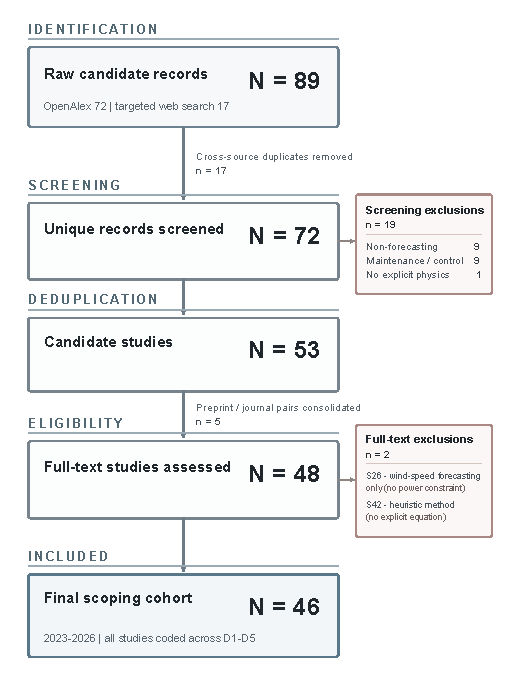
\includegraphics[width=0.85\textwidth]{figure2.pdf}
 \caption{Ultra-LSNT architecture. A decomposition module separates trend and seasonal components. Multi-scale temporal embeddings (e.g., $k=3$ and $k=7$ kernels for wind) feed a sparse MoE encoder. A Jump Gate optionally skips redundant computation. Conditional execution reduces average compute and supports energy-aware edge-constrained inference (lower energy per sample inference under the profiling protocol in Table~\ref{tab:efficiency}).}
 \label{fig:architecture}
\end{figure}


\noindent\textbf{Series decomposition for robust representation.} 
Wind power series typically contain both slow-varying trends (meteorology-driven) and fast seasonal/fluctuation components (turbulence, wake effects, measurement noise). Related decomposition--fusion pipelines and hybrid attention models have been widely reported in Applied Energy for renewable and multi-energy forecasting \cite{li2023novel,ma2022hybrid}. We employ a moving-average decomposition:
\begin{equation}
\mathbf{X} = \mathbf{X}_{\text{trend}} + \mathbf{X}_{\text{season}}, \qquad 
\mathbf{X}_{\text{trend}} = \text{MA}(\mathbf{X}),
\end{equation}
where $\text{MA}(\cdot)$ is a moving average operator. The trend branch captures low-frequency structure with minimal capacity, while the seasonal branch is handled by the sparse MoE to focus computation on the hard nonlinear part.


\noindent\textbf{Multi-scale temporal embedding.}\label{sec:embedding}
A key difficulty in wind power forecasting is the coexistence of short-term turbulence and medium-range regime shifts. To model heterogeneous temporal scales without over-parameterizing, we construct multi-scale temporal embeddings via 1D convolutions:
\begin{equation}
\mathbf{E}_s = \text{Conv1D}_{k_s}(\mathbf{X}_{\text{season}}), \qquad
\mathbf{E}_m = \text{Conv1D}_{k_m}(\mathbf{X}_{\text{season}}),
\end{equation}
followed by fusion:
\begin{equation}
\mathbf{E} = \phi\big(\mathbf{W}_s\mathbf{E}_s + \mathbf{W}_m\mathbf{E}_m\big),
\end{equation}
where $\phi(\cdot)$ denotes a nonlinearity (e.g., GELU), and $\mathbf{W}_s,\mathbf{W}_m$ are learnable projections. In the wind dataset ablation, we adopt $k_m=7$ as the default medium-scale kernel (the selection rationale is reported in the ablation section), while $k_s$ remains small to preserve short-range responsiveness.

This embedding is intentionally convolutional rather than attention-heavy. Recent SOTA forecasters often rely on patching and attention-based encoders (e.g., PatchTST and iTransformer) that excel when long-range token mixing is affordable \cite{nie2023patchtst,liu2024itransformer}. In contrast, SCADA streams exhibit high-frequency turbulence bursts and short-range wake effects where a local receptive field is a natural inductive bias; multi-scale kernels cover both fast and medium dynamics without forcing global attention at every step. From a deployment standpoint, Conv1D maps cleanly to highly optimized dense primitives on edge CPUs/NPUs/DSPs, yielding predictable memory access and latency profiles, whereas attention kernels can incur higher overhead due to data-dependent indexing and quadratic token mixing \cite{zhou2019edge,strubell2019energy,schwartz2020greenai}. We therefore use convolutional embeddings to front-load edge efficiency, while leaving regime diversity and longer-range adaptation to sparse expert routing in the MoE encoder.


\noindent\textbf{Sparse Mixture-of-Experts encoder.}\label{sec:moe}
Let $\mathbf{e}_t$ be the embedded token at time $t$. We employ $N$ experts $\{E_i(\cdot)\}_{i=1}^{N}$, each a lightweight feed-forward module:
\begin{equation}
E_i(\mathbf{e}_t)=\sigma(\mathbf{W}_i\mathbf{e}_t+\mathbf{b}_i),
\end{equation}
where $\sigma(\cdot)$ is an activation function.

\paragraph{Top-$K$ routing.}
A router produces probabilities over experts:
\begin{equation}
\mathbf{p}_t = \text{Softmax}(\mathbf{W}_r\mathbf{e}_t + \boldsymbol{\epsilon}),
\end{equation}
where $\boldsymbol{\epsilon}$ denotes small injected noise to encourage exploration during training. The Top-$K$ gate selects the set $\mathcal{S}_t$ of $K$ experts with the highest probabilities. The sparse MoE output is:
\begin{equation}
\mathbf{h}_t = \sum_{i\in\mathcal{S}_t} p_{t,i}\,E_i(\mathbf{e}_t).
\end{equation}
This conditional computation is the core mechanism that jointly serves robustness (specialization and noise filtering) and sustainability (reduced average FLOPs and energy).


\subsection{Edge-oriented optimization and training}
\label{subsec:method_edge_train}


\noindent\textbf{Edge deployment constraint: compute vs. storage.} Sparse MoE reduces average computation by activating only $K$ experts per input, but edge devices are often constrained by memory capacity and storage bandwidth. Ultra-LSNT therefore uses MoE primarily for \emph{functional decoupling} rather than unlimited capacity scaling: experts specialize to distinct operating regimes (e.g., stable conditions, drift, and high-frequency measurement noise), while Top-$K$ routing activates only the relevant experts to provide \emph{on-demand robustness}. To make the edge claim falsifiable, we report both the \emph{active} compute path (Top-$K$ routing) and the full footprint (parameter count and checkpoint size; Table~\ref{tab:efficiency}). The Lite family further compresses the sparse module by reducing MoE depth/width and using Top-$1$ routing (Eq.~\ref{sec:edge}), explicitly targeting RAM/flash constraints in addition to FLOPs.

\noindent\textbf{Training objective and routing stability.}\label{sec:objective}
We optimize mean squared error for point forecasting:
\begin{equation}
\mathcal{L}_{\text{pred}} = \frac{1}{H}\sum_{h=1}^{H}\left\|\hat{y}_{t+h}-y_{t+h}\right\|_2^2.
\end{equation}
\noindent\textbf{Optional uncertainty indicators and probabilistic head.}
Although we report point metrics in the main results, the MoE structure naturally supports uncertainty-aware operation with minimal overhead. 
A simple structural indicator is the router entropy $H_t=-\sum_{i=1}^{N}p_{t,i}\log(p_{t,i}+\epsilon)$, where higher entropy suggests weaker specialization for the current input.
A complementary indicator is expert disagreement within the active set $\mathcal{S}_t$, computed as the sample variance of expert outputs $\{\hat{y}^{(i)}_{t+h}\}_{i\in\mathcal{S}_t}$ for each horizon step $h$.
These indicators can be used for conservative control logic (e.g., disabling skipping in Jump Gate, or increasing reserve margins) without requiring distributional training targets.

When probabilistic supervision is desired, the same backbone can be equipped with an output head that predicts either (i) quantiles $\{\hat{y}^{(q)}\}$ trained with pinball loss (with $\mathcal{Q}$ denoting a quantile set, e.g., $\{0.1,0.5,0.9\}$), or (ii) Gaussian parameters $(\mu,\sigma)$ trained by negative log-likelihood:
\begin{equation}
\mathcal{L}_{\text{pin}}=\frac{1}{|\mathcal{Q}|H}\sum_{q\in\mathcal{Q}}\sum_{h=1}^{H}\rho_q\!\left(y_{t+h}-\hat{y}^{(q)}_{t+h}\right),\quad
\rho_q(e)=\max(qe,(q-1)e),
\end{equation}
\begin{equation}
\mathcal{L}_{\text{nll}}=\frac{1}{H}\sum_{h=1}^{H}\left(\frac{(y_{t+h}-\mu_{t+h})^2}{2\sigma_{t+h}^2}+\log\sigma_{t+h}\right).
\end{equation}
We include these formulations to facilitate risk-aware extensions (e.g., PICP/PINAW/CRPS reporting), while keeping the core edge-oriented encoder and routing mechanisms unchanged.

To prevent expert collapse and to stabilize routing under non-ideal inputs (e.g., sensor drift or low-bit quantization), we add a load-balancing regularizer:

\begin{equation}
\mathcal{L}_{\text{aux}} = \sum_{i=1}^{N}\left(\bar{p}_i - \frac{1}{N}\right)^2,\qquad
\bar{p}_i=\frac{1}{T}\sum_{t=1}^{T}p_{t,i},
\end{equation}
and the final objective:
\begin{equation}
\mathcal{L} = \mathcal{L}_{\text{pred}} + \lambda\,\mathcal{L}_{\text{aux}}.
\end{equation}
In the released implementation, the router adopts a conservative default \texttt{aux\_loss\_coef} of $\lambda=0.01$ to regularize expert utilization; we treat $\lambda$ as a task-dependent hyperparameter and report its sensitivity for deployment guidance. Concretely, we evaluate $\lambda\in\{0.00,0.01,0.05,0.10\}$ under the same validation protocol (Table~\ref{tab:ablation_lambda}) and observe that $\lambda=0.05$ yields the highest $R^{2}$ (0.8832), whereas weaker regularization ($\lambda=0.01$) degrades $R^{2}$ to 0.8715 and overly strong regularization ($\lambda=0.10$) reduces $R^{2}$ to 0.8731. This helps interpret the sensitivity results that follow. For the cross-model comparisons and robustness benchmarks reported in this paper, we keep the conservative default $\lambda=0.01$ to avoid introducing additional tuning degrees of freedom beyond those available to baseline models, while the $\lambda$ sweep is provided to enable practitioners to retune routing stability for their sensing and operational regimes (e.g., drift-prone sensors, low-bit quantization, or noisy telemetry). A controlled robustness check (Table~\ref{tab:lambda_robust_compare} shows that $\lambda=0.01$ and $0.05$ yield very similar robustness at $\sigma_{\mathrm{eff}}\in\{0.30,0.60\}$ (|$\Delta R^2$| $\leq 0.0027$). We therefore keep $\lambda=0.01$ as the released default configuration and treat $\lambda=0.05$ as an optional tuning setting rather than a different method variant.

Accordingly, all headline benchmark tables use checkpoints trained with $\lambda=0.01$; the $\lambda$ sweep is reported strictly as sensitivity evidence and deployment-oriented guidance, rather than as tuned results. Taken together, this motivates the next step. To close the loop on this choice, we additionally conduct a controlled robustness comparison between $\lambda\in\{0.01,0.05\}$ at two representative noise levels ($\sigma_{\mathrm{eff}}\in\{0.30,0.60\}$). Both variants follow the same initialization and training pipeline (a quick controlled fine-tune; only $\lambda$ differs), and we log routing statistics alongside accuracy.

\begin{table}[t]
\centering
\caption{Controlled robustness comparison for the router regularization coefficient $\lambda$ at two representative noise severities on Wind (CN). $R^2$ is evaluated under the same train-fitted z-score inverse-scaling protocol and the same noise definition (in normalized space) used in Table~\ref{tab:robust_gaussian_sweep}. The $\lambda=0.05$ row is obtained via a controlled fine-tune from the main checkpoint (5 epochs; AdamW lr=$5\times10^{-5}$, wd=$0.01$; same split/scaler), while $\lambda=0.01$ uses the released default checkpoint. Expert usage variance summarizes the variability of expert selection proportions (lower indicates more uniform usage).}
\label{tab:lambda_robust_compare}
\begin{tabular}{lcccc}
\toprule
$\lambda$ & $R^2$ @ $\sigma_{\mathrm{eff}}=0.30$ & $R^2$ @ $\sigma_{\mathrm{eff}}=0.60$ & Usage var @ 0.30 & Usage var @ 0.60 \\
\midrule
0.01 & 0.8544 & 0.7295 & 0.0405 & 0.0407 \\
0.05 & 0.8518 & 0.7322 & 0.0378 & 0.0380 \\
\bottomrule
\end{tabular}
\end{table}


\noindent\textbf{End-to-end procedures and reproducibility.}\label{sec:algo_summary}
For review convenience and reproducibility, we summarize the end-to-end pipeline in Algorithm~\ref{alg:train} (training with imperfection injection) and Algorithm~\ref{alg:infer} (edge inference with Jump Gate). Fig.~\ref{fig:workflow} provides a compact workflow view from SCADA measurements to dispatch outcomes.

\begin{algorithm}[t]
\caption{Ultra-LSNT training with SCADA imperfection injection}
\label{alg:train}
\begin{algorithmic}[1]
\STATE \textbf{Input:} training samples $(\mathbf{X},\mathbf{Y})$ with $\mathbf{X}\in\mathbb{R}^{L\times C}$, $\mathbf{Y}\in\mathbb{R}^{H\times 1}$
\STATE \textbf{Hyperparameters:} experts $N$, Top-$K$, router regularizer $\lambda$, noise config $\sigma_{\mathrm{cfg}}$, industrial scale $\alpha$, Jump Gate threshold $\tau$
\STATE $\sigma_{\mathrm{eff}} \leftarrow \alpha \cdot \sigma_{\mathrm{cfg}}$
\STATE $\tilde{\mathbf{X}} \leftarrow \mathrm{InjectImperfections}(\mathbf{X}; \sigma_{\mathrm{cfg}},\sigma_{\mathrm{eff}})$
\STATE \hspace{1em}\textit{(Gaussian noise, drift, quantization; see Sec.~\ref{sec:robust_protocol} for definitions.)}
\STATE $(\mathbf{X}_{\mathrm{trend}},\mathbf{X}_{\mathrm{resid}}) \leftarrow \mathrm{Decompose}(\tilde{\mathbf{X}})$
\STATE $\mathbf{Z} \leftarrow \mathrm{MultiScaleEmbed}([\mathbf{X}_{\mathrm{trend}},\mathbf{X}_{\mathrm{resid}}])$
\FOR{$b=1$ \TO $N_{\mathrm{blk}}$}
 \STATE $\mathbf{g}\leftarrow \mathrm{Router}_b(\mathbf{Z})$ \hspace{1em}\textit{(routing probabilities)}
 \STATE $\mathcal{E}\leftarrow \mathrm{TopK}(\mathbf{g},K)$ \hspace{1em}\textit{(selected experts)}
 \STATE $\mathbf{Z}\leftarrow \mathrm{AggregateExperts}_b(\mathbf{Z},\mathcal{E})$
 \STATE $\mathbf{Z}\leftarrow \mathbf{Z} + \mathrm{TrendInteract}_b(\mathbf{Z},\mathbf{X}_{\mathrm{trend}})$
\ENDFOR
\STATE $\hat{\mathbf{Y}} \leftarrow \mathrm{ForecastHead}(\mathbf{Z})$
\STATE $\mathcal{L}_{\mathrm{pred}} \leftarrow \mathrm{MSE}(\hat{\mathbf{Y}},\mathbf{Y})$
\STATE $\mathcal{L}_{\mathrm{aux}} \leftarrow \mathrm{LoadBalance}(\mathbf{g})$
\STATE Update parameters to minimize $\mathcal{L}_{\mathrm{pred}} + \lambda\,\mathcal{L}_{\mathrm{aux}}$
\end{algorithmic}
\end{algorithm}
\begin{algorithm}[t]
\caption{Edge inference with Jump Gate}
\label{alg:infer}
\begin{algorithmic}[1]
\STATE \textbf{Input:} window $\mathbf{X}\in\mathbb{R}^{L\times C}$
\STATE $(\mathbf{X}_{\mathrm{trend}},\mathbf{X}_{\mathrm{resid}}) \leftarrow \mathrm{Decompose}(\mathbf{X})$
\STATE $\mathbf{Z} \leftarrow \mathrm{MultiScaleEmbed}([\mathbf{X}_{\mathrm{trend}},\mathbf{X}_{\mathrm{resid}}])$
\FOR{$b=1$ \TO $N_{\mathrm{blk}}$}
 \IF{$\mathrm{JumpGate}_b(\mathbf{Z};\tau)=\mathrm{SKIP}$}
 \STATE \textbf{continue}
 \ENDIF
 \STATE Route experts and aggregate as in Algorithm~\ref{alg:train}
\ENDFOR
\STATE $\hat{\mathbf{Y}} \leftarrow \mathrm{ForecastHead}(\mathbf{Z})$
\STATE \textbf{Output:} $\hat{\mathbf{Y}}$
\end{algorithmic}
\end{algorithm}
\begin{figure}[t]
\centering
\IfFileExists{workflow_pipeline.pdf}{%
 \includegraphics[width=0.95\textwidth]{workflow_pipeline.pdf}%
}{%
 \fbox{\parbox{0.95\textwidth}{\centering \textbf{Workflow placeholder.}\\
 Suggested content: SCADA imperfections $\rightarrow$ Ultra-LSNT forecasting $\rightarrow$ edge metrics (latency/size/energy proxy) $\rightarrow$ dispatch optimization $\rightarrow$ cost/reserve/curtailment.}}%
}
\caption{Dispatch-economic outcomes under forecast uncertainty: total operating cost, reserve burden, and curtailment sensitivity across forecast quality levels.}
\label{fig:workflow}
\end{figure}


\noindent\textbf{Edge-ready acceleration: Jump Gate and Ultra-LSNT-Lite.}\label{sec:edge}
\paragraph{Jump Gate for dynamic skipping.}
Not every time step requires equal computation. We introduce a Jump Gate that computes an importance score $I_t$:
\begin{equation}
I_t = \text{Sigmoid}(\mathbf{w}_g^\top \mathbf{e}_t),
\end{equation}
and conditionally skips the MoE update when the token is deemed redundant:
\begin{equation}
\mathbf{h}_t =
\begin{cases}
\mathbf{h}_{t-1}, & I_t < \tau, \\
\text{MoE}(\mathbf{e}_t), & \text{otherwise},
\end{cases}
\end{equation}
where $\tau$ is a threshold. This mechanism provides a conservative, controllable skipping policy. In our CPU batch-1 benchmark, wall-clock latency differences across $\tau$ are within run-to-run variance, so we interpret the skip rate primarily as a computation-path indicator; larger savings are expected on platforms where the MoE update dominates runtime.

\noindent\textbf{Differentiable training and ramp-safety.} During training, the hard threshold in the Jump Gate can be replaced by a smooth relaxation to keep the objective fully differentiable: $\tilde z_t=\sigma\big((I_t-\tau)/s\big)$ with temperature $s>0$, and the block update becomes $\mathbf{h}_t = \tilde z_t\cdot\mathrm{MoE}(\mathbf{e}_t) + (1-\tilde z_t)\cdot\mathbf{h}_{t-1}$. This yields $\partial \tilde z_t/\partial I_t = \tilde z_t(1-\tilde z_t)/s$ and allows standard backpropagation. At inference, we apply the conservative hard-threshold policy. To avoid information loss during rapid ramps, $\tau$ can be set conservatively (or the gate can be disabled by a simple local ramp detector), and we report $\tau$ sensitivity and skip rates to make the trade-off explicit (Table~\ref{tab:tau_sweep_pareto}).


\paragraph{Ultra-LSNT-Lite for sustainable deployment.}
To further reduce carbon and cost of inference, we derive Ultra-LSNT-Lite by compressing the sparse module while keeping the decomposition and multi-scale embedding backbone. Concretely, we reduce MoE depth and width and use Top-$1$ routing, which preserves expert specialization but minimizes dispatch overhead:
\begin{equation}
(N,K,\text{\#MoE blocks},d) \ \rightarrow \ (2,1,1,96),
\end{equation}
where $d$ is the hidden dimension. The design is motivated by edge constraints (memory, thermal envelope, and power budget) and by responsible AI deployment practices: smaller models reduce operational emissions and broaden access to reliability-focused forecasting without requiring large compute infrastructure.


\noindent\textbf{Complexity considerations.}\label{sec:complexity}
Let $d$ denote hidden dimension. A dense $N$-expert computation scales as $\mathcal{O}(N\cdot L \cdot d^2)$, whereas Top-$K$ routing reduces it to $\mathcal{O}(K\cdot L \cdot d^2)$ with $K\ll N$. Jump Gate further reduces the effective token count by skipping low-importance steps, providing an additional multiplicative reduction in average cost. These properties are crucial for grid-edge scenarios where both reliability and energy efficiency are first-order requirements.


\section{Experimental Setup}
\label{sec:design}

This section specifies the empirical settings in a reproducible manner, including data sources, preprocessing, baselines, evaluation metrics, and protocols for robustness and deployment-oriented efficiency assessment. Following standard practice, we focus this section on what is evaluated and how, and defer the why to Results and Discussion. 

\subsection{Data description and preprocessing}

\subsubsection{Primary wind power forecasting case}
Our primary case study is an ultra-short-term wind power forecasting task built upon real-world supervisory control and data acquisition (SCADA) measurements from a utility-scale wind farm in Xinjiang, China. The task reflects operational forecasting needs under realistic sensor uncertainty and non-stationary atmospheric conditions. To support interpretability analysis later, the input variables include physically meaningful signals (e.g., wind speed-related and environment-related measurements), and the target is the aggregated active power output.

\begin{table}[t]
\centering
\caption{Summary of the primary Wind (CN) SCADA dataset and task definition used in this manuscript.}
\label{tab:data_summary_windcn}
\begin{tabular}{p{0.33\linewidth}p{0.60\linewidth}}
\toprule
Item & Value \\
\midrule
Data source & Utility wind farm SCADA (anonymized; publicly released) \\
Sampling interval & 15\,min \\
Time span & 2021-04-02 00:00 to 2022-06-30 23:45 \\
Aggregation level & SCADA record level from one wind farm (asset identifiers anonymized) \\
Target & Active power (\texttt{power}), unit: kW; normalization to rated power: No (z-score fitted on train split only) \\
Input features & 8 variables: \texttt{windspeed}, \texttt{power}, \texttt{winddirection}, \texttt{temperature}, \texttt{humidity}, \texttt{pressure}, \texttt{windspeed\_round\_0.1}, \texttt{power\_round\_1} (rounded auxiliaries emulate SCADA rounding/quantization; provided to all models for a fair comparison) \\
Missing/outlier handling & Duplicate/non-numeric columns removed; columns with $>$30\% missing dropped; linear interpolation + bfill/ffill applied within each split (after chronological split) to avoid train--test leakage; NaN/Inf sanity checks; modeling columns missing rate: core channels 0.00\%, rounded auxiliary channels 0.18\% \\
Train/test split & 80\% / 20\% chronological (97,222 / 24,306 records) \\
Train/Test date ranges & Train: 2021-04-02 00:00 to 2022-03-12 15:45; Test: 2022-03-12 16:00 to 2022-06-30 23:45 \\
Lookback / horizon & $L=96$ steps, $H=24$ steps \\
Hourly variant for dispatch & For Section~\ref{subsec:results_dispatch}, we construct an hourly series by averaging each 4 consecutive 15-min records and use $L=96,H=24$ on the 1h grid (4 days lookback, 24h horizon). \\
\bottomrule
\end{tabular}
\end{table}
\begin{figure}[t]
 \centering
 \includegraphics[width=\linewidth]{data_statistics_2x2_real.pdf}
 \caption{Representative raw series excerpt of the primary wind power case. The figure is intended to provide visual grounding for seasonality, ramps, and intermittency that motivate robustness-oriented modeling.}
 \label{fig:data_statistics}
\end{figure}
\subsubsection{Multi-domain validation tasks}
To examine whether the proposed architecture generalizes beyond a single site and a single physical process, we further evaluate on three heterogeneous forecasting tasks, covering wind power from another region, environmental monitoring, and electricity demand. Concretely, we report results on \emph{Wind (US)}, \emph{Air Quality}, and \emph{GEFCom Load} in addition to \emph{Wind (CN)}. These datasets span different sampling frequencies, noise characteristics, and dynamic regimes, which makes them suitable for testing cross-domain robustness and transferability without task-specific architectural modification.

\subsubsection{Chronological splitting and normalization}
To prevent temporal leakage and reflect real deployment where future data are unavailable during training, all datasets are split strictly by time order. For the primary Wind (CN) benchmark in this manuscript, we use a chronological 80\%/20\% split (97,222/24,306 records). Some training scripts additionally carve out an internal validation subset from the training partition for early stopping. Z-score normalization is always fitted on training data only, and the same transformation is applied to evaluation data. For error metrics reported in physical units, predictions and targets are inverse-transformed before metric computation to ensure comparability across models and datasets.

\subsubsection{Data quality control and robust loading}
Because energy and environmental time series often contain missing values, duplicated columns, timestamp artifacts, and non-numeric placeholders, we apply a consistent data quality control pipeline before modeling. The pipeline removes duplicate and non-numeric columns, performs linear interpolation for missing values, and enforces sanity checks for NaN/Inf as well as minimum sample-size constraints. These steps are implemented as part of the project's robust data-loading utilities, ensuring that all experiments use the same validated inputs and improving reproducibility under real-world data imperfections.

\subsection{Benchmark models and comparison scope}

The baseline set is designed to cover a representative spectrum of forecasting philosophies that are commonly used in energy forecasting practice: attention-based Transformers for long-range dependency modeling (Informer \cite{zhou2021informer}, Autoformer \cite{wu2021autoformer}), recent strong patching/mixing designs (PatchTST \cite{nie2023patchtst}, TimeMixer \cite{wang2024timemixer}), emerging efficient backbones (iTransformer \cite{liu2024itransformer}, Mamba (S6) \cite{gu2023mamba}, DLinear \cite{zeng2023dlinear}), and a widely adopted tree-based operational baseline (LightGBM \cite{ke2017lightgbm}). This coverage enables us to analyze not only point-forecast accuracy, but also how different modeling paradigms trade robustness against deployment realism under sensor perturbations.

\subsection{Evaluation metrics}

We evaluate point forecasting accuracy using $R^2$, RMSE, and MAE as the primary evidence, which reflect goodness-of-fit and absolute error in dataset-native physical units.
We additionally define MAPE for completeness; however, for wind power series with frequent near-zero generation periods, ratio-based errors can be disproportionately inflated even with numerical safeguards, so we treat MAPE as a supplementary diagnostic rather than a headline metric.

\begin{equation}
R^2 = 1 - \frac{\sum_{t=1}^{T}(y_t - \hat{y}_t)^2}{\sum_{t=1}^{T}(y_t - \bar{y})^2}, 
\quad
\text{RMSE} = \sqrt{\frac{1}{T}\sum_{t=1}^{T}(y_t - \hat{y}_t)^2},
\end{equation}
\begin{equation}
\text{MAE} = \frac{1}{T}\sum_{t=1}^{T}|y_t - \hat{y}_t|,
\quad
\text{MAPE} = \frac{100}{T}\sum_{t=1}^{T}\left|\frac{y_t - \hat{y}_t}{y_t + \epsilon}\right|.
\end{equation}
Here $\bar{y}$ is the sample mean of $y_t$, and $\epsilon$ is a small constant used to avoid numerical instability when $y_t$ approaches zero.

\noindent\textbf{Operationally oriented diagnostics.}
Average errors can hide tail risk and timing errors that are critical in dispatch and ramp management. 
To complement $R^2$/RMSE/MAE, we include in the supplementary evidence package (i) tail errors such as the 95th percentile and maximum absolute error, and (ii) a ramp-aware score that evaluates detection and magnitude errors on large power changes within a short window.
We also report (iii) forecast smoothness via the total variation of the predicted trajectory and (iv) routing stability via the Jaccard similarity of the Top-$K$ expert sets across adjacent windows, as abrupt switching can be undesirable in downstream control.
For probabilistic variants (Section~\ref{sec:objective}), standard interval and distribution scores such as PICP, PINAW, and CRPS can be reported using the same inverse-scaling chain.

\subsection{Robustness evaluation overview}
\label{sec:robust_protocol}
We evaluate reliability under three SCADA-style imperfections: additive measurement noise, calibration drift, and quantization. To avoid unit ambiguity, severity is reported relative to the clean signal scale (e.g., as a fraction of the signal standard deviation for additive noise). The Gaussian noise sweep spans mild to severe conditions up to 60\% of the clean standard deviation; drift and quantization use aligned severity grids. Full perturbation definitions, parameter grids, and implementation notes are provided in Appendix~\ref{app:robust_details}.

\noindent\textbf{Fairness and training regime.}
Unless explicitly stated, all models are trained on the same clean training split with identical normalization, and perturbations are applied only at inference time to the inputs while targets remain unperturbed. 
This design probes \emph{inherent} robustness to SCADA imperfections rather than robustness obtained by model-specific noise augmentation. 
All reported $R^2$/RMSE/MAE values are computed after inverse scaling using the same target-column statistics to ensure a consistent evaluation chain.

\subsection{Deployment-oriented efficiency measurement and Green AI reporting}

A key motivation of this work is to support edge-constrained forecasting where efficiency translates into lower operational energy consumption and improved accessibility for resource-constrained operators. Therefore, we report latency, model size and parameter count for the proposed model family under a fixed-shape profiling protocol; the batch size used for each measurement is reported together with the results. For Ultra-LSNT-Lite, we additionally provide an energy estimate based on average device power and average forward time ($E_{\text{fwd}}=\bar{P}\cdot\bar{t}$), and report the per-sample equivalent $E_{\text{inf}}=E_{\text{fwd}}/B$ for transparency.

This reporting practice aligns with ``Green AI'' principles \cite{schwartz2020greenai,strubell2019energy} by making the computational footprint an explicit part of the empirical evidence, rather than an implicit assumption. It also supports responsible deployment considerations in energy systems: compact models reduce hardware requirements and can be deployed closer to the data source, which may improve data governance and privacy by minimizing raw-data transfer to the cloud. The final plots used in the manuscript are generated through the project's consolidated figure scripts (e.g., multi-domain plots, expert heatmaps, and dispatch comparison charts), ensuring that all visual evidence is traceable to logged experimental outputs.

\subsection{Downstream dispatch optimization setup}
\label{subsec:dispatch_setup}
To align the downstream study with State Grid provincial day-ahead (DA) dispatch practice, we formulate the DA scheduling problem over a 24-hour horizon with 1-hour granularity (DA, 24h, 1h resolution)\cite{dlt5002_2021}. We summarize forecast-driven operational impact using three operator-facing indicators: (i) total operating cost (thermal energy, reserve procurement, and penalty terms), (ii) total wind curtailment, and (iii) feasibility stability measured by the frequency of feasibility-restoration (fallback) events. All monetary outcomes are reported in CNY in the main text; if a USD conversion is required in the editorial workflow, we will use the annual-average exchange rate of the corresponding year and report the conversion rate explicitly.

As a network-consistency supplement, we retain a two-stage day-ahead/real-time (DA/RT) DC-OPF study on IEEE RTS-24, and report network-facing indicators including total slack, congestion ratio, and (when logged) OPF success ratio.

To quantify the operational value of forecasts, we couple point forecasts to a simplified day-ahead dispatch model (24-hour horizon) with a thermal unit, upward reserve procurement, and an energy storage device, following practices that map forecast errors to operating cost in grid operations \cite{botterud2011operational,yan2025economicvalue}. Let $\hat{w}_t$ denote the wind power forecast (kW), $d_t$ the demand (kW), and define dispatch variables: thermal output $g_t$ (kW), procured upward reserve $r_t$ (kW), wind curtailment $u_t$ (kW), storage charge/discharge power $p_{\text{ch},t},p_{\text{dis},t}$ (kW), and state-of-charge $s_t$ (kWh). \textbf{Time-grid alignment.} The dispatch model is formulated on a 1\,h grid. We therefore construct an hourly variant of Wind (CN) by averaging each 4 consecutive 15-min SCADA records (Table~\ref{tab:data_summary_windcn}). Ultra-LSNT is trained on this hourly series with $L=96,H=24$ and outputs a 24-step hourly forecast vector $\hat{w}_{1:24}$, which is used directly as the dispatch input. With $\Delta t=1$\,h and a horizon $T=24$, each forecaster produces a 24-step hourly wind vector $\hat{w}_{1:T}$ (kW) that feeds the dispatch engine. We evaluate a 120-day rolling window for Ultra-LSNT and representative baselines (iTransformer, TimeMixer, and DLinear), and report the frequency of \emph{feasibility-restoration (fallback)} events (fraction of days tagged as \texttt{fallback\_x0} in our implementation). A fallback day indicates that the dispatch instance requires the fallback feasibility mapping (Eq.~\ref{eq:dispatch_feas_map}) to recover a feasible schedule, and is therefore interpreted as an \emph{operational feasibility-domain stability} indicator. This copper-plate formulation does not include explicit transmission limits; accordingly, fallback is not a direct congestion metric.

\noindent\textbf{Feasibility-restoration events as an operational stability indicator.}
In our implementation, a day is tagged as \texttt{fallback\_x0} when the dispatch optimizer requires a conservative fallback initialization to recover a feasible schedule under the same algebraic constraints; this reflects how close the forecast-driven dispatch instance is to the feasibility boundary in our workflow, rather than a physical transmission-constraint violation.

\noindent\textbf{Forecast-to-dispatch scaling.}
To align forecast magnitudes with the dispatch operating range, we record and release the forecast scaling metadata used in the rolling study (see \texttt{dispatch\_rolling\_with\_ultra\_scaled\_meta.json}). In the logged configuration, a global affine mapping transforms the wind series from the observed range $[14250,131839]$ to the dispatch range $[20000,40000]$ (kW) before applying the feasibility mapping below.

To keep the feasible operating region consistent across models in the rolling setting, we apply a deterministic feasibility mapping to each daily forecast vector:
\begin{equation}
\tilde{w}_t=\mathrm{clip}(s\hat{w}_t,0,w_{\max}),\qquad
s=\min\left(1,\frac{w_{\max}}{\max_t \hat{w}_t + \epsilon}\right),
\label{eq:dispatch_feas_map}
\end{equation}
where $w_{\max}=\max(w_{\text{train}})$ is computed on the hourly training split and $\epsilon$ is a small constant. Results under this mapping are reported in Table~\ref{tab:dispatch_rolling}; the raw-forecast rolling summary is included in the supplementary evidence package.

\begin{align}
\min_{\cdot}\quad C_{\text{dispatch}} &= C_{\text{fuel}} + C_{\text{reserve}} + C_{\text{purchase}} + C_{\text{storage}} + C_{\text{startup}} + C_{\text{shutdown}}, \label{eq:dispatch_obj}\\
C_{\text{fuel}} &= c_f\sum_{t=1}^{T} g_t\Delta t,\qquad
C_{\text{reserve}} = c_r\sum_{t=1}^{T} r_t\Delta t, \nonumber\\
C_{\text{purchase}} &= c_f\sum_{t=1}^{T} p_{\text{ch},t}\Delta t,\qquad
C_{\text{storage}} = c_s\sum_{t=1}^{T} p_{\text{dis},t}\Delta t, \nonumber\\
C_{\text{startup}} &= c_{\text{su}}\sum_{t=2}^{T}\frac{\max(g_t-g_{t-1},0)}{R_{\max}},\quad
C_{\text{shutdown}} = c_{\text{su}}\sum_{t=2}^{T}\frac{\max(g_{t-1}-g_t,0)}{R_{\max}}, \nonumber
\end{align}
subject to power balance and operational constraints:
\begin{align}
& g_t + \hat{w}_t + p_{\text{dis},t} - p_{\text{ch},t} - u_t = d_t,\quad 0\le u_t \le \hat{w}_t,\quad \forall t, \label{eq:dispatch_balance}\\
& g_{\min}\le g_t\le g_{\max},\quad 0\le r_t,\quad g_t+r_t\le g_{\max},\quad |g_t-g_{t-1}|\le R_{\max}, \label{eq:dispatch_gen}\\
& 0\le p_{\text{ch},t}\le P_{\text{ch},\max},\quad 0\le p_{\text{dis},t}\le P_{\text{dis},\max}, \label{eq:dispatch_storage_power}\\
& s_t = s_{t-1} + \eta_{\text{ch}}p_{\text{ch},t}\Delta t - \eta_{\text{dis}}^{-1}p_{\text{dis},t}\Delta t,\quad 0\le s_t\le S_{\max}. \label{eq:dispatch_storage_soc}
\end{align}
All monetary coefficients are in Chinese Yuan (CNY) as implemented in \texttt{evaluate\_cost}. Since the absolute magnitude depends on the chosen price coefficients and a reference year, we focus on unitless comparisons (relative reductions against a fixed baseline) in addition to the absolute values in Table~\ref{tab:dispatch_rolling}; this makes the conclusions invariant to exchange rates and simple rescaling. With $\Delta t=1$\,h, summations of kW schedules correspond to kWh energy over the horizon. We compute costs and dispatch metrics using the realized wind output on the same test day consistently for all forecasting models (see \texttt{compare\_dispatch\_metrics.py} and \texttt{wind\_dispatch\_model.py}).

\begin{table}[t]
\centering
\caption{Dispatch model parameters used in the 120-day rolling day-ahead evaluation. Power quantities are in kW; reserve and curtailment are accumulated energy in kWh. Monetary coefficients are in Chinese Yuan (CNY) as implemented; no currency conversion is applied.}
\label{tab:dispatch_params}
\begin{tabular}{ll}
\toprule
Parameter & Value \\
\midrule
Time resolution / horizon & $\Delta t=1$\,h; $T=24$ (rolling evaluation) \\
Demand profile $d_t$ & Fixed demand of 50{,}000\,kW (constant across $t$) \\
Wind uncertainty rule & $\sigma_{w,t}=0.2\cdot|\hat{w}_t|$ (kW), applied per time step \\
Thermal generation bounds & $g_{\min}=10{,}000$\,kW; $g_{\max}=80{,}000$\,kW \\
Thermal ramp constraint & $R_{\max}=20{,}000$\,kW/h \\
Fuel cost & 0.5 CNY/kWh \\
Startup cost coefficient $c_{\text{su}}$ & 5{,}000 CNY per start \\
Shutdown cost coefficient & Same as $c_{\text{su}}$ (implementation uses startup\_cost) \\
Reserve cost & 0.2 CNY/kWh (reserve capacity) \\
Storage energy capacity & $S_{\max}=50{,}000$\,kWh \\
Storage power limits & $P_{\text{ch},\max}=10{,}000$\,kW; $P_{\text{dis},\max}=10{,}000$\,kW \\
Storage efficiencies & $\eta_{\text{ch}}=0.95$; $\eta_{\text{dis}}=0.95$ \\
Storage operating cost & 0.05 CNY/kWh \\
Initial state of charge & $\text{SOC}_0=0.5$ (fraction of $S_{\max}$) \\
\bottomrule
\end{tabular}
\end{table}

\noindent\textbf{Note on network constraints.}
The dispatch model above is a single-node (copper-plate) formulation intended to isolate how forecast errors propagate to reserve, curtailment, and operating cost under a transparent parameterization. To address reviewer concerns on transmission realism, we additionally run a network-constrained DC-OPF benchmark on IEEE RTS-24 using PYPOWER (\texttt{rundcopf}), with explicit line thermal limits and archived wind-bus mapping metadata (\texttt{results/supplementary\_evidence/dispatch\_network\_ieee24\_dcopf\_wmax260\_meta.json}).

\subsection{Reproducibility statement}
All experiments are executed under a unified training and evaluation pipeline with fixed preprocessing, chronological splitting, and consistent metric computation. To make the study reproducible and auditable, we report the full computational environment and training configurations in Appendix~\ref{app:impl_details}, and we keep the plotting scripts aligned with logged outputs so that all tables and figures are traceable to deterministic evaluation code.

To facilitate independent reproduction, the full source code (including model definition, perturbation generators, and evaluation scripts) is publicly released at \url{https://github.com/b1ue13e/Ultra-LSNT} under the MIT license. The repository includes a pinned \texttt{requirements.txt}, step-by-step commands to reproduce each main table/figure, and the full imperfection injection scripts (noise, drift, and quantization), including the multi-seed sanity checks used to validate robustness behavior. For exact reproducibility, we recommend that readers cite the repository together with a specific commit hash corresponding to the submission version (or a tagged release when available), so the same dependency graph and implementation details can be recovered.

The primary Wind (CN) SCADA dataset is released publicly to support full reproducibility and independent verification. Nevertheless, the complete preprocessing and evaluation protocol is fully specified in this manuscript and implemented in the released codebase, enabling reproduction on public benchmarks and facilitating on-site verification for partners with access to similar SCADA telemetry.

\subsection{Implementation summary}
We release the full codebase (model, perturbation generators, and evaluation scripts) and provide sufficient protocol detail for independent reproduction on public benchmarks. Software/hardware specifications and configuration tables are reported in Appendix~\ref{app:impl_details}.

\section{Results}
\label{sec:results}
%========================
This section reports evidence in the order an operator would typically care about it: baseline accuracy, stability under sensing imperfections, and transfer across related energy/environmental tasks, followed by edge-deployment footprint and downstream dispatch value. Unless otherwise stated, RMSE/MAE are computed after inverse scaling in the original units of each dataset; they therefore complement the scale-free $R^2$.


\subsection{Predictive performance and stability analysis}
\label{subsec:results_main}
%----------------------------------------
Table~\ref{tab:main_wind_cn} reports clean-setting point-forecast accuracy on Wind (CN) after inverse scaling. For transparency and fair comparison, Ultra-LSNT is evaluated using the conservative router regularization default $\lambda=0.01$ throughout the benchmark tables; $\lambda$ sensitivity is analyzed separately in Section~\ref{subsec:results_ablation}. In the \emph{clean-measurement} setting, DLinear ranks highest on Wind~(CN). We additionally report a non-learned Persistence baseline (last-value predictor) to contextualize the dataset difficulty; it is competitive on this short-horizon setting, but it provides no learned representation and is therefore used only as a sanity-check reference.
 This is informative but incomplete for operations: strong clean accuracy can coexist with brittle behavior once sensing quality degrades. Ultra-LSNT attains $R^2=0.8728$---lower than the clean leader yet competitive with several deep baselines---and is explicitly designed to avoid catastrophic degradation under realistic SCADA imperfections (Section~\ref{subsec:results_robustness}).

\begin{table}[t]
\centering
\caption{Main forecasting performance on Wind (CN). Metrics are computed after inverse scaling using the train-fitted z-score; RMSE/MAE are reported in kW. (Higher $R^2$ is better; lower RMSE/MAE are better).}
\label{tab:main_wind_cn}
\begin{tabular}{lccc}
\toprule
Model & $R^2$ & RMSE & MAE \\
\midrule
DLinear & \textbf{0.9400} & \textbf{6236.39} & \textbf{4085.09} \\
Persistence (na\"ive) & 0.9175 & 7313.94 & 4760.16 \\
Mamba (S6) & 0.9208 & 7165.88 & 4875.17 \\
iTransformer (arXiv 2023) & 0.9012 & 8004.05 & 6333.29 \\
TimeMixer (ICLR 2024) & 0.8886 & 8498.38 & 6661.36 \\
Ultra-LSNT (Ours) & 0.8728 & 9080.55 & 7171.42 \\
PatchTST (ICLR 2023) & 0.8666 & 9298.08 & 7342.16 \\
Informer & 0.8167 & 10900.65 & 8765.92 \\
Autoformer & 0.7219 & 13424.28 & 10646.77 \\
\bottomrule
\end{tabular}
\end{table}

\begin{figure}[t]
\centering
\includegraphics[width=\linewidth]{Figure_3_Final.pdf}
\caption{Time-series zoom-in of representative forecast trajectories on Wind (CN), highlighting local trend tracking and ramp-following behavior.}
\label{fig:fig3_main_comparison}
\end{figure}


\noindent\textbf{Robustness to measurement perturbations.}\label{subsec:results_robustness}
We evaluate universal robustness by injecting perturbations only at inference time on the test split, while keeping the same normalization/denormalization and metric pipeline as in Table~\ref{tab:main_wind_cn}. Severity is reported by the effective noise ratio $\sigma_{\mathrm{eff}}=\alpha\sigma_{\mathrm{cfg}}$ with $\alpha=1.5$ (Section~3.4.1), so a configured $\sigma_{\mathrm{cfg}}=0.40$ corresponds to an effective $\sigma_{\mathrm{eff}}=0.60$ corruption in the normalized space.

\noindent\textbf{Universal Gaussian noise stress test on Wind (CN).}\label{subsubsec:universal_noise}
Table~\ref{tab:robust_gaussian_sweep} reports a sweep over configured $\sigma_{\mathrm{cfg}}\in\{0.00,0.10,0.20,0.30,0.40\}$ (effective ratios shown in parentheses) for Ultra-LSNT, DLinear, LightGBM, and a non-learned Persistence baseline (last-value predictor) as a sanity check. The operational signal is the degradation trajectory: the strongest clean learned baseline (DLinear) deteriorates sharply as noise increases, while Ultra-LSNT degrades more gradually and stays positive under severe corruption. Persistence remains comparatively stable under Gaussian noise on Wind~(CN), which reflects strong short-horizon autocorrelation and motivates reporting it explicitly.


\begin{table}[t]
\centering
\caption{Gaussian-noise robustness sweep on Wind (CN). We report both the configured noise ratio $\sigma_{\mathrm{cfg}}$ (used by our scripts) and the corresponding effective ratio $\sigma_{\mathrm{eff}}=\alpha\sigma_{\mathrm{cfg}}$ with $\alpha=1.5$. Injected noise uses std $\sigma_{\mathrm{eff}}\cdot\mathrm{std}(x)$. Metrics use the same inverse-scaling evaluation pipeline as Table~\ref{tab:main_wind_cn}. For DLinear, multi-seed verification at representative settings confirms systematic degradation under strong noise: $R^2=0.2908\pm0.0045$ at $\sigma_{\text{cfg}}=0.20$ and $R^2=-1.6482\pm0.0149$ at $\sigma_{\text{cfg}}=0.40$ (5 seeds), with $R^2<0$ indicating worse performance than the mean predictor.}
\label{tab:robust_gaussian_sweep}
\begin{tabular}{lcccc}
\toprule
$\sigma_{\mathrm{cfg}}$ ($\sigma_{\mathrm{eff}}$) & Ultra-LSNT $R^2$ & DLinear $R^2$ & LightGBM $R^2$ & Persistence $R^2$ \\
\midrule
0.00 (0.00) & 0.8728 & \textbf{0.9400} & 0.9069  & 0.9175 \\
0.10 (0.15) & 0.8687 & 0.7814 & 0.8860  & 0.9140 \\
0.20 (0.30) & 0.8552 & 0.2952 & 0.8222  & 0.9034 \\
0.30 (0.45) & 0.7866 & -0.4659 & 0.7305  & 0.8879 \\
0.40 (0.60) & 0.7263 & -1.5790 & 0.6156  & 0.8612 \\
\bottomrule
\end{tabular}
\end{table}

\begin{table}[t]
\centering
\caption{Compact efficiency--robustness summary on Wind (CN). ``Noisy'' corresponds to the Gaussian perturbation level $\sigma_{\mathrm{cfg}}=0.20$ (effective $\sigma_{\mathrm{eff}}=0.30$ after scaling). CPU latency uses batch size $B=1$ measurements from Table~\ref{tab:cpu_batch1_latency}. Parameter counts for neural models are from Table~\ref{tab:efficiency}; LightGBM is reported as an FP32-equivalent count converted from the measured 27.18\,MiB serialized artifact.}
\label{tab:eff_robust_tradeoff}
\scriptsize
\begin{tabular}{lccccc}
\toprule
Model & Params (M) & Latency (ms) & Clean $R^2$ & Noisy $R^2$ & $R^2$ drop (\%) \\
\midrule
DLinear & 0.21 & 0.213 & 0.9400 & 0.2952 & 68.6 \\
LightGBM & 7.12 & 50.215 & 0.9069 & 0.8222 & 9.3 \\
Ultra-LSNT & 34.46 & 3.714 & 0.8728 & 0.8552 & 2.0 \\
\bottomrule
\end{tabular}
\end{table}



\noindent\textbf{Two-point robustness summary.} At $\sigma_{\mathrm{cfg}}=0.20$ (i.e., $\sigma_{\mathrm{eff}}=0.30$ with $\alpha=1.5$), Ultra-LSNT degrades by only 2.01\% in $R^2$ (0.8728$\rightarrow$0.8552), versus 9.35\% for LightGBM (0.9069$\rightarrow$0.8222) and 68.60\% for DLinear (0.9400$\rightarrow$0.2952). This indicates that the released default configuration (including $\lambda=0.01$) prioritizes operational stability under realistic sensing perturbations. In particular, Ultra-LSNT surpasses the clean leader DLinear already at $\sigma_{\mathrm{eff}}=0.15$ (i.e., $\sigma_{\mathrm{cfg}}=0.10$), indicating that the robustness crossover occurs at mild corruption levels that are plausible in field telemetry.

\noindent\textbf{Interpreting negative $R^2$ under extreme stress.} A negative $R^2$ means the mean squared error exceeds the variance of the target ($R^2=1-\mathrm{MSE}/\mathrm{Var}$), so performance is worse than a naive mean predictor under that stress configuration. In our protocol, all models are trained on the same clean training split and then evaluated under \emph{unseen} input corruption without retraining, to emulate unexpected SCADA imperfections at deployment. Although linear mappings do not create deep nonlinear amplification, they also lack a mechanism to separate corrupted regimes: severe perturbations shift the input distribution and can distort the trend/seasonal components that linear forecasters rely on, producing large systematic errors. Ultra-LSNT mitigates this distribution shift through sparse conditional routing and expert specialization, which acts as a set of regime-specific predictors and reduces worst-case failures. Training-time noise augmentation for each baseline is a separate design choice and is not the focus here; the goal is to compare inherent robustness under a unified evaluation pipeline.

\begin{figure}[htbp]
 \centering
 \includegraphics[width=0.85\linewidth]{robustness_curve.pdf}
 \caption{Robustness under progressively increasing additive Gaussian noise on Wind (CN). Ultra-LSNT overtakes the clean leader DLinear at mild corruption ($\sigma_{\mathrm{eff}}=0.15$) and degrades more slowly thereafter. The x-axis corresponds to the configured ratio $\sigma_{\mathrm{cfg}}$ in our scripts; the effective injected standard deviation is $\sigma_{\mathrm{eff}}=\alpha\sigma_{\mathrm{cfg}}$ ($\alpha=1.5$), relative to $\mathrm{std}(x)$.}
 \label{fig:robust_gaussian_sweep}
\end{figure}


\noindent\textbf{Drift and quantization perturbations.}
Beyond additive Gaussian noise, we evaluate \emph{drift} and \emph{quantization} perturbations using the explicit, reproducible protocols in Section~3.4.2. Drift is implemented as a persistent random-walk bias added to each channel, while quantization is implemented as step-size rounding with $\Delta=\sigma_{\mathrm{eff}}\cdot \mathrm{std}(x)$. Figure~\ref{fig:robustness_drift_quant} summarizes the results over configured $\sigma_{\mathrm{cfg}}\in\{0.00,0.10,0.20,0.30,0.40\}$ (effective $\sigma_{\mathrm{eff}}\in\{0.00,0.15,0.30,0.45,0.60\}$). Drift yields a clear monotonic degradation as severity increases, reflecting sensitivity to slowly accumulating bias, whereas step-size quantization produces a comparatively milder impact within the tested range.


\noindent\textbf{Missingness and imputation artifacts.}
SCADA streams commonly experience dropouts (e.g., communication loss or sensor resets) followed by simple imputation in the data pipeline. We emulate this by masking inputs at rate $p\in\{0.1,0.3\}$ and applying either forward-fill (\texttt{ffill}) or linear interpolation before inference. Table~\ref{tab:robust_missingness} reports mean$\pm$std over three seeds. As missingness increases from $p=0.1$ to $p=0.3$, both models degrade, but the change is smaller for Ultra-LSNT: its $R^2$ decreases by about 0.002--0.003 with modest RMSE growth, whereas DLinear exhibits a larger $R^2$ drop and a sharper RMSE increase under the same imputation settings.

\begin{table}[t]
\centering
\caption{Robustness under missingness and simple imputation on Wind (CN) (3 seeds; mean$\pm$std). $p$ denotes the missing rate and imputation is applied along the time axis before inference.}
\label{tab:robust_missingness}
\begin{tabular}{lccccc}
\toprule
Imputation & $p$ & Ultra-LSNT $R^2$ & Ultra-LSNT RMSE (kW) & DLinear $R^2$ & DLinear RMSE (kW) \\
\midrule
\texttt{ffill} & 0.1 & $0.8718\pm0.0001$ & $9115.0\pm3.6$ & $0.9326\pm0.0001$ & $6610.9\pm4.4$ \\
\texttt{ffill} & 0.3 & $0.8692\pm0.0002$ & $9205.8\pm8.4$ & $0.9242\pm0.0005$ & $7010.0\pm23.9$ \\
\texttt{linear} & 0.1 & $0.8722\pm0.0001$ & $9102.4\pm2.9$ & $0.9325\pm0.0001$ & $6613.6\pm6.0$ \\
\texttt{linear} & 0.3 & $0.8705\pm0.0002$ & $9162.9\pm6.9$ & $0.9239\pm0.0006$ & $7021.1\pm27.9$ \\
\bottomrule
\end{tabular}
\end{table}

\begin{figure}[htbp]
 \centering
 \includegraphics[width=0.90\linewidth]{drift_quant_results.pdf}
 \caption{Robustness stress-test summary on Wind (CN), comparing degradation trends under progressively harsher SCADA-style perturbations.}
 \label{fig:robustness_drift_quant}
\end{figure}


\noindent\textbf{Generalization across heterogeneous domains.}\label{subsec:results_generalization}
Table~\ref{tab:multi_domain} reports Ultra-LSNT performance across four domains. We report errors in dataset-native units (after inverse scaling) together with the Jump Gate skip rate as an optional deployment knob. In the main Wind (CN) setting we use a conservative threshold $\tau$ so that skipping is rare (accuracy-first), while conditional computation primarily comes from sparse Top-$K$ expert routing. Overall, the same architecture remains functional beyond Wind (CN) without task-specific redesign: it attains low error on Wind (US) with a moderate skip rate, and maintains stable behavior (near-zero skipping) on Air Quality and GEFCom Load under the fixed threshold $\tau$. The absolute error levels differ by domain, which is expected given heterogeneous data-generating processes and covariate availability.

\begin{table}[t]
\centering
\caption{Cross-domain generalization comparison using $R^2$ (higher is better). We use $R^2$ here because it is invariant to affine re-scaling of the target and thus avoids unit/scale ambiguity across heterogeneous datasets. The last column reports the Jump Gate skip rate for Ultra-LSNT under the released default threshold $\tau$ (accuracy-first).}
\label{tab:multi_domain}
\begin{tabular}{lcccc}
\toprule
Dataset & Ultra-LSNT $R^2$ & DLinear $R^2$ & TimeMixer $R^2$ & Ultra skip rate (\%) \\
\midrule
Wind (CN) & 0.8728 & 0.9400 & 0.8886 & 0.0 \\
Wind (US) & 0.7878 & 0.8796 & 0.8023 & 11.4 \\
Air Quality & 0.4861 & 0.3400 & 0.3869 & 0.0 \\
GEFCom Load & 0.7554 & 0.7363 & 0.7271 & 0.0 \\
\bottomrule
\end{tabular}
\end{table}

\paragraph{Cross-domain metric choice.}
Absolute error metrics (RMSE/MAE) depend on dataset units and scaling, which can easily create apparent inconsistencies across heterogeneous domains if evaluation pipelines differ. Therefore, we use $R^2$ in Table~\ref{tab:multi_domain} as the primary cross-domain comparison metric (scale-invariant under affine re-scaling). For interpretability, Table~\ref{tab:multi_domain_baselines} reports Ultra-LSNT dataset-native RMSE/MAE after inverse scaling, along with the corresponding skip rate under the released default $\tau$.

\begin{table}[t]
\centering
\caption{Auxiliary dataset-native error metrics for Ultra-LSNT after inverse scaling (reported in original units of each dataset). This table complements Table~\ref{tab:multi_domain}, which uses $R^2$ for scale-invariant cross-domain comparison.}
\label{tab:multi_domain_baselines}
\begin{tabular}{lcccc}
\toprule
Dataset & RMSE & MAE & Unit & Skip rate (\%)\\
\midrule
Wind (CN) & 9081 & 7171 & kW & 0.0 \\
Wind (US) & 0.4556 & 0.2891 & MW & 11.4 \\
Air Quality & 32.21 & 19.87 & AQI & 0.0 \\
GEFCom Load & 2837 & 2049 & MW & 0.0 \\
\bottomrule
\end{tabular}
\end{table}

We additionally report the skip rate of Jump Gate in Table~\ref{tab:multi_domain} to clarify when conditional computation yields measurable savings. The skip rate varies by domain: it is non-zero on Wind (US), while it is near zero on Wind (CN), Air Quality, and GEFCom Load under the fixed threshold $\tau$. This indicates that the model conservatively chooses full computation in higher-volatility or lower signal-to-noise regimes, rather than forcing aggressive skipping that could harm reliability-sensitive energy operations. In other words, Jump Gate is designed as a ``do no harm'' mechanism: it skips computation when the regime is stable, and defaults to full computation when uncertainty is high.

\begin{figure}[t]
\centering
\includegraphics[width=\linewidth]{fig_multi_domain.pdf}
\caption{Multi-domain generalization visualization across four datasets.}
\label{fig:multi_domain_fig}
\end{figure}


\paragraph{Domain interpretation.}\label{subsec:disc_generalization}
The multi-domain evaluation indicates that Ultra-LSNT maintains reasonable predictive capability across wind power, air quality, and load forecasting, despite substantial differences in dynamics and measurement processes. This supports the claim that the method is not narrowly tuned to a single dataset artifact.

At the same time, the domain gap in $R^2$ highlights that generalization is conditional on the signal characteristics. Air quality forecasting, for instance, often involves stronger exogenous drivers, delayed effects, and non-local transport phenomena; a purely data-driven temporal model may require richer covariates or domain-informed structure to close the gap. For energy applications, this observation motivates a cautious interpretation: multi-domain robustness is encouraging, but domain-specific error modes still require diagnosis before deployment.


\noindent\textbf{Sensitivity analyses, interpretability, and statistical checks.}\label{subsec:results_ablation_summary}
We keep the main text focused on deployment-relevant evidence and summarize controlled sensitivities for key design choices (e.g., decomposition scale and routing regularization). Detailed ablation tables are provided in Appendix~\ref{app:supp_tables}.

\paragraph{Interpretability as auditability.}\label{subsec:results_interpret}
Sparse routing yields expert-usage logs that can be inspected alongside physical covariates, supporting auditability in safety-critical forecasting. Expert-specialization tables and visualizations are provided in Appendix~\ref{app:supp_tables}.

\paragraph{Statistical checks.}\label{subsec:results_significance_summary}
We report significance checks as supplementary evidence; Diebold--Mariano test tables are provided in Appendix~\ref{app:supp_tables}.

\paragraph{Interpretability for safety-critical use.}\label{subsec:disc_interpretability}
The expert specialization analysis shows that different experts correlate with distinct physical drivers (e.g., wind speed, turbulence, temperature, humidity). This is not merely a visualization result; it implies that the model's internal decision pathways can be audited in physically meaningful terms.

In safety-critical energy operations, auditability is a deployment requirement. When forecasts are used downstream (e.g., reserve sizing or curtailment decisions), operators need to understand when the model is reacting to plausible meteorological cues versus when it might be responding to artifacts. Expert-level signals provide a structured interface for such inspection: abnormal activation patterns can be used as early warnings for sensor faults or regime shifts, supporting responsible and transparent AI use in critical systems.



\noindent\textbf{Ramp sensitivity, tail risk, and forecast smoothness.}
Average-error summaries can mask ramp misses and heavy-tailed errors that drive operational risk. We therefore evaluate diagnostics on the $t+1$ (15-min) stream. Ramp events are defined on a 1-hour window ($4\times$15\,min) using $|\Delta_{1h}|\ge 0.05\,P_{\max}$, where $P_{\max}=\max(y_{\text{true}})=131{,}839$\,kW (threshold 6{,}591.95\,kW). Table~\ref{tab:ramp_tail_smoothness} reports tail errors, ramp-event F1, and total variation (TV) as a smoothness proxy. On the clean stream, DLinear shows smaller tail errors and higher ramp-event F1, consistent with its higher clean-data point-forecast accuracy. Ultra-LSNT produces a markedly lower TV (TV/TV$_{\text{true}}$ well below 1), indicating a conservative, low-jitter trajectory; this helps suppress spurious high-frequency oscillations that can propagate into downstream decision-making. Router diagnostics (variance, max-share, entropy) indicate stable expert utilization without collapse, supporting the claim that conditional computation is active and well-behaved. We also include a simple static ensemble (0.5 Ultra-LSNT + 0.5 DLinear) to probe whether the observed behavior can be replicated by fixed-weight averaging. Since the robustness claims in Tables~\ref{tab:robust_gaussian_sweep} and~\ref{tab:eff_robust_tradeoff} hinge on stability under measurement imperfections, we treat the ramp--smoothness balance as a task-specific tuning dimension rather than a single objective to optimize in isolation.

\begin{table}[t]
\centering
\caption{Ramp/tail/smoothness diagnostics on Wind (CN) using the 15-min $t+1$ forecast stream. Ramp events are defined by $|\Delta_{1h}|\ge 0.05\,P_{\max}$ with $P_{\max}=131{,}839$\,kW (threshold 6{,}591.95\,kW). TV is $\sum_t | \hat{y}_t-\hat{y}_{t-1} |$; TV/TV$_{\text{true}}$ normalizes by the realized series. Routing stability is reported for Ultra-LSNT via the mean router-usage variance (lower is more stable), together with the mean max-share and normalized entropy of routing weights.}
\label{tab:ramp_tail_smoothness}
\begin{tabular}{lrrrrrrr}
\toprule
Model & $P95(|e|)$ (kW) & $\max(|e|)$ (kW) & Ramp F1 & TV (kW) & TV/TV$_{\text{true}}$ & Routing var & (max-share, entropy) \\
\midrule
Ultra-LSNT & 11,940.17 & 34,544.14 & 0.3544 & 8,222,569.29 & 0.2525 & 0.04413 & (0.5394, 0.7511) \\
DLinear & 2,484.47 & 21,479.02 & 0.5939 & 29,013,519.33 & 0.8909 & --- & --- \\
Static ensemble (0.5U+0.5D) & 6,151.70 & 28,011.58 & 0.5000 & 15,059,403.24 & 0.4624 & --- & --- \\
\bottomrule
\end{tabular}
\end{table}

\noindent\textbf{Minimal probabilistic baseline (post-hoc Gaussian calibration).}
To respond to the increasing emphasis on uncertainty quantification, we report a minimal probabilistic baseline obtained by post-hoc Gaussian calibration on the clean test split: $\mu=\hat{y}$ and a constant $\sigma$ estimated as the residual standard deviation. Table~\ref{tab:prob_gaussian_minimal} reports Gaussian NLL, CRPS, and interval coverage/width at nominal 80\% and 90\% levels. As expected, these scores largely track deterministic error: DLinear yields smaller residual variance and closer-to-nominal coverages with narrower intervals. Ultra-LSNT shows under-coverage, suggesting heavier-tailed and nonstationary residuals that are not captured by a constant-$\sigma$ Gaussian. This highlights the need for a learned, heteroscedastic output head (e.g., quantiles or $\mu,\sigma$) and proper probabilistic objectives (CRPS/pinball), which we treat as future work rather than a prerequisite for the robustness evidence reported above.

\begin{table}[t]
\centering
\caption{Post-hoc Gaussian calibration baseline on Wind (CN) (clean test split). We set $\mu=\hat{y}$ and estimate a constant $\sigma$ as the residual standard deviation on the evaluation stream. PICP and PINAW are reported for nominal 80\% and 90\% prediction intervals.}
\label{tab:prob_gaussian_minimal}
\begin{tabular}{lrrrrrr}
\toprule
Model & $\sigma$ (kW) & NLL & CRPS & PICP@80 / PINAW@80 & PICP@90 / PINAW@90 \\
\midrule
Ultra-LSNT & 5,044.08 & 10.1314 & 3,353.4667 & 0.7253 / 0.10995 & 0.8242 / 0.14111 \\
DLinear & 1,329.74 & 8.6118 & 670.2737 & 0.8726 / 0.02898 & 0.9269 / 0.03720 \\
\bottomrule
\end{tabular}
\end{table}


\subsection{Computational efficiency for edge deployment}
\label{subsec:results_efficiency}
%----------------------------------------
From a Green-AI perspective, reporting forecasting accuracy together with computational footprint is useful for energy applications that increasingly run analytics on power- and memory-constrained hardware. In this work we avoid board-level power claims and instead report a reproducible \emph{energy proxy} derived from CUDA-synchronized runtime under a fixed reference power envelope. Specifically, we define the batch-normalized proxy $E_{\text{inf}}=\bar{P}_{\text{ref}}\cdot\bar{t}/B$, where $\bar{t}$ is the mean forward latency and $\bar{P}_{\text{ref}}=150$~W is used only for normalization. For a deployment device with average power $\bar{P}_{\text{dev}}$, the implied electricity attributable to inference scales linearly by $\bar{P}_{\text{dev}}/\bar{P}_{\text{ref}}$, so the daily inference electricity can be approximated as
\begin{align}
\text{kWh/day} \approx \frac{E_{\text{inf}} \cdot N_{\text{call}}}{3.6\times 10^{9}}\cdot\frac{\bar{P}_{\text{dev}}}{\bar{P}_{\text{ref}}}.
\end{align}
Given an actual device power envelope and grid emission factor, the same scaling yields a Scope-2 CO$_2$e estimate for comparing alternatives under identical call rates. As an order-of-magnitude example, for $N_{\text{turb}}=100$ turbines and one forecast every 5 minutes ($N_{\text{call}}=28{,}800$ per day), the Lite (opt.) proxy $E_{\text{inf}}=0.038$~mJ/sample implies negligible electricity even after rescaling, suggesting that real-time latency and memory footprint are more likely to be binding constraints than the proxy electricity itself.

\textbf{What ``Lite (opt.)'' means.} Ultra-LSNT-Lite (opt.) combines three reproducible optimizations: (i) a reduced architecture (hidden\_dim=96, num\_blocks=1, num\_experts=2, top\_k=1), (ii) \texttt{torch.compile(mode='max-autotune')} to enable kernel fusion and autotuned execution, and (iii) CUDA AMP \texttt{autocast} for mixed-precision (FP16) inference. We do \emph{not} use INT8 quantization, ONNX/TensorRT, or vendor-specific graph compilers in these numbers. Model ``Size'' refers to the serialized on-disk weight artifact produced by the above settings (without optimizer states).
Table~\ref{tab:efficiency} reports deployment-facing footprint evidence from a fixed-shape GPU microbenchmark (RTX~4090). For Ultra-LSNT-Lite, energy is estimated as $E_{\text{fwd}}=\bar{P}\cdot\bar{t}$ per forward call and converted to a per-sample value $E_{\text{inf}}=E_{\text{fwd}}/B$ using the profiling batch size ($B=256$); we report both for transparency. The optimized Ultra-LSNT-Lite reduces the fp32 footprint to 1.33\,MiB and achieves 6.53\,ms per forward call, corresponding to an estimated $E_{\text{inf}}=0.038$\,mJ per sample on this setup.

From a Green-AI perspective, these measurements turn efficiency into first-class empirical evidence: forecasting is executed repeatedly across fleets of turbines or substations, so per-inference energy and memory footprint accumulate into operational overhead and indirect emissions depending on the electricity mix. Reporting these numbers also improves responsible deployment practice, because operators can explicitly trade accuracy against compute/energy budgets rather than relying on implicit engineering assumptions. Table~\ref{tab:cpu_batch1_latency} reports CPU batch-1 latency for the Ultra-LSNT family (full / Lite / Lite(opt.)) together with representative baselines, under a single-thread setting (warm-up + repeated runs). This demonstrates that the Ultra-LSNT family can run under an online inference regime ($B=1$) within practical real-time budgets, complementing the GPU throughput profiling in Table~\ref{tab:efficiency}. We do not claim to beat linear models on absolute latency; the claim is robust real-time feasibility under realistic sensing imperfections.

We emphasize that these efficiency results should be interpreted through the lens of \emph{robust efficiency}: linear models are fastest on any hardware, but their robust accuracy can be unacceptable under realistic imperfections; Ultra-LSNT aims to stay within real-time budgets while maintaining reliability.

\begin{table}[t]
\centering
\caption{Efficiency profiling on a fixed-shape GPU microbenchmark (RTX~4090). These numbers are intended as a throughput reference and may differ on edge CPUs/ARM devices and under batch-1 online inference. ``Latency'' is the average wall-clock time per forward call (batch size $B$ shown; CUDA-synchronized with warm-up). ``Checkpoint file size'' is the on-disk size of the weights-only serialized artifact produced by \texttt{torch.save} (zipfile-based serialization; no optimizer states); it is not the raw parameter byte count and can differ from a naive FP32/FP16 estimate. Energy is reported only for Ultra-LSNT-Lite variants as an \emph{energy proxy}: $E_{\text{fwd}}=\bar{P}\cdot\bar{t}$ with a fixed reference power $\bar{P}=150$~W and the measured mean forward latency $\bar{t}$; the batch-normalized proxy is $E_{\text{inf}}=E_{\text{fwd}}/B$. Energy scales linearly with $\bar{P}$; readers can rescale to their target device power envelope. This is a reproducible proxy for relative comparison, not a board-level power measurement.}
\label{tab:efficiency}
\begin{tabular}{lcccccc}
\toprule
Model & Params (M) & Checkpoint file size (MiB) & $B$ & Latency / forward (ms) & $E_{\text{fwd}}$ (mJ) & $E_{\text{inf}}$ (mJ/sample) \\
\midrule
Ultra-LSNT & 34.46 & 131.62 & 128 & 18.84 & -- & -- \\
Ultra-LSNT-Lite (orig.) & 1.34 & 5.10 & 256 & 10.42 & 13.41 & 0.052 \\
Ultra-LSNT-Lite (opt.) & 0.35 & 1.33 & 256 & 6.53 & 9.80 & 0.038 \\
DLinear & 0.21 & 0.80 & 128 & 0.05 & -- & -- \\
TimeMixer & 2.60 & 9.91 & 128 & 7.27 & -- & -- \\
\bottomrule
\end{tabular}
\end{table}

\begin{table}[t]
\centering
\caption{CPU microbenchmark at batch size $B=1$ (single-sample online inference) on the same host CPU, with \texttt{threads=1}, \texttt{warmup=50}, and \texttt{measure=250}. Latency is reported as mean $\pm$ std over repeated runs; throughput is $1/\text{latency}$.}
\label{tab:cpu_batch1_latency}
\begin{tabular}{lcc}
\toprule
Model & Latency (ms) & Throughput (Hz) \\
\midrule
Ultra-LSNT (full) & 3.714 $\pm$ 0.341 & 269.3 \\
Ultra-LSNT-Lite (orig.) & 2.430 $\pm$ 0.245 & 411.5 \\
Ultra-LSNT-Lite (opt.) & 1.171 $\pm$ 0.201 & 854.0 \\
DLinear & 0.2654 $\pm$ 0.0843 & 3767.6 \\
LightGBM & 50.3970 $\pm$ 21.1347 & 19.8 \\
\bottomrule
\end{tabular}
\end{table}

\begin{figure}[t]
\centering
\includegraphics[width=0.98\linewidth]{fig_pareto_latency_rmse_lite.pdf}
\caption{Pareto trade-off between inference latency and point-forecast error on Wind (CN). Latency is measured with batch size $=1$ on CPU (Table~\ref{tab:cpu_batch1_latency}); RMSE is computed after inverse scaling on the same test split. The optimized Lite configuration improves the accuracy--efficiency balance compared with the original Lite setting.}
\label{fig:pareto_lite}
\end{figure}



\noindent\textbf{ARMv8 single-core benchmark.}
To bridge the gap between workstation microbenchmarks and realistic edge hardware, we additionally run a single-core ARMv8
(aarch64) benchmark on a Huawei Kunpeng~920 CPU using the same batch-$1$ inference setting.
Ultra-LSNT (Full) achieves an average latency of $3.275$~ms (P95 $4.349$~ms), while Ultra-LSNT-Lite achieves $2.348$~ms (P95 $3.137$~ms).
The corresponding serialized model artifacts are $1.021$~MB and $0.154$~MB, respectively (measured after export to the deployment format used in the benchmark script).
The benchmark script and raw logs are included in the repository for reproducibility (Table~\ref{tab:arm_microbenchmark}).


\begin{table}[t]
\centering
\caption{ARMv8 single-core microbenchmark (Huawei Kunpeng~920, aarch64, batch-$1$). Reported values are mean and P95 latency after warm-up; artifact size is measured on the serialized deployment format used by \texttt{benchmark\_arm.py}.}
\label{tab:arm_microbenchmark}
\begin{tabular}{lccc}
\toprule
Model & Avg latency (ms) & P95 latency (ms) & Artifact size (MB) \\
\midrule
Ultra-LSNT (Full) & 3.275 & 4.349 & 1.021 \\
Ultra-LSNT-Lite & 2.348 & 3.137 & 0.154 \\
\bottomrule
\end{tabular}
\end{table}

\begin{figure}[t]
\centering
\includegraphics[width=\linewidth]{fig_efficiency.pdf}
\caption{Efficiency comparison visualization. GPU throughput profiling and the energy proxy are reported in Table~\ref{tab:efficiency}; CPU batch-1 latency is reported in Table~\ref{tab:cpu_batch1_latency}.}
\label{fig:efficiency_fig}
\end{figure}


\paragraph{Why explicit footprint reporting matters.}\label{subsec:disc_greenai}
A central contribution of this work is treating computational footprint as first-order evidence rather than an implicit side note. Table~\ref{tab:efficiency} makes this point concrete: the optimized Ultra-LSNT-Lite (Opt.) reduces the fp32 footprint from 5.10\,MiB to 1.33\,MiB and decreases the average per-forward latency from 10.42\,ms to 6.53\,ms. Under the same profiling batch size ($B=256$), the estimated per-forward energy decreases from 13.41\,mJ to 9.80\,mJ (per-sample equivalent: 0.052\,$\rightarrow$\,0.038\,mJ). Because this per-sample value is obtained by dividing a batch microbenchmark ($B=256$), it should be interpreted as an optimistic lower bound relative to batch-1 online inference. This shows that a compressed variant can better match tight deployment budgets while preserving the core modeling structure.

These reductions matter for ``Green AI'' evaluation because forecasting is executed repeatedly across fleets of assets. In such settings, energy per sample inference and memory footprint accumulate into operational overhead and, depending on the electricity mix, indirect emissions. Although absolute energy values are hardware-dependent, explicitly reporting energy per sample inference and storage turns sustainability and deployability into measurable, comparable criteria rather than implicit assumptions.

Edge-ready execution can also support data governance by reducing the need for continuous raw SCADA transmission to remote services, which may lower exposure of operational data streams and align with data-minimization or policy-compliant deployment in critical infrastructure. This governance benefit is not automatic---it depends on the surrounding security controls and access policies---but local inference expands the feasible design space for responsible deployment.

Finally, the Lite compression trade-off suggests an actionable workflow: a full-capacity model can serve as a reference and training anchor, while a compressed variant is tuned to site-specific edge constraints with bounded performance degradation. This suggests that a compressed variant can better match edge constraints in practice, while keeping performance within an acceptable range.


\noindent\textbf{Jump Gate as an optional efficiency knob.}
To make the reliability--efficiency trade-off explicit on Wind (CN), we run a threshold sweep $\tau\in\{0.3,0.5,0.7,0.9\}$ and report the resulting accuracy, skip rate, and CPU batch-1 latency (Table~\ref{tab:tau_sweep_pareto}); Fig.~\ref{fig:tau_sweep_pareto} visualizes the Pareto frontier.


\begin{table}[t]
\centering
\caption{Jump Gate threshold ($\tau$) sweep on Wind (CN), illustrating the accuracy--skipping trade-off under CPU batch-1 inference (single thread). RMSE is in kW after inverse scaling.}
\label{tab:tau_sweep_pareto}
\begin{tabular}{lcccc}
\toprule
$\tau$ & $R^2$ & RMSE (kW) & Skip rate (\%) & CPU latency (ms) \\
\midrule
0.3 & 0.8661 & 9314.40 & 33.38 & 3.621 \\
0.5 (default) & 0.8728 & 9081.66 & 0.00 & 3.628 \\
0.7 & 0.8728 & 9081.66 & 0.00 & 3.766 \\
0.9 & 0.8728 & 9081.66 & 0.00 & 3.665 \\
\bottomrule
\end{tabular}
\end{table}

\begin{figure}[t]
\centering
\includegraphics[width=0.90\linewidth]{tau_sweep_ultra_pareto_v3.pdf}
\caption{Accuracy--skipping trade-off of Jump Gate on Wind (CN) under a $\tau$ threshold sweep (CPU batch-1).}
\label{fig:tau_sweep_pareto}
\end{figure}

On Wind (CN), the Jump Gate behaves conservatively at the default threshold ($\tau=0.5$), with near-zero skip rate. This indicates an accuracy-first ``do-no-harm'' regime: when uncertainty is high, the model prefers full computation instead of aggressive skipping. Meaningful skipping appears only at a lower threshold ($\tau=0.3$; skip rate 33.38\%), while the latency gain is bounded by runtime overhead. Therefore, we keep $\tau=0.5$ as the default for reliability-oriented deployment, and treat lower-$\tau$ settings as optional efficiency tuning.


\subsection{Economic benefits in power dispatch}
\label{subsec:results_dispatch}
%----------------------------------------
We evaluate whether forecasting behavior translates into operational value via a day-ahead dispatch optimization on an hourly variant of Wind (CN) (Section~\ref{subsec:dispatch_setup}). We run a 120-day rolling simulation where each model supplies a 24-step hourly wind forecast per day, and summarize total operating cost and curtailment over the full horizon, together with the frequency of feasibility-restoration (fallback) events, which we interpret as an operational feasibility-domain stability indicator.

Table~\ref{tab:dispatch_rolling} summarizes the rolling outcomes under the feasibility mapping in Eq.~\ref{eq:dispatch_feas_map}. Relative to DLinear, Ultra-LSNT reduces the 120-day total operating cost from 54.47M to 35.97M~CNY (33.96\% reduction) and cuts total curtailment from 55.71M to 22.09M~kWh (60.35\% reduction). All three deep baselines (iTransformer, TimeMixer, Ultra-LSNT) substantially lower both cost and curtailment compared with DLinear, and they also exhibit far fewer fallback days (i.e., higher operational feasibility rates). Under this simplified setting, load shedding does not occur for any model; the main economic signal is therefore driven by the interaction between forecast errors, reserve procurement, and curtailment decisions.

Assuming this 120-day window is representative of annual operation, the observed Ultra-LSNT vs.\ DLinear gap implies an annualized operating-cost saving of approximately 56.26M~CNY and an annualized curtailment reduction of approximately 102.26~GWh. These values are scenario-based extrapolations under the fixed dispatch parameterization rather than guaranteed plant-level outcomes.




\begin{table}[t]
\centering
\caption{Rolling dispatch evaluation over 120 days on the hourly Wind (CN) setting (fixed demand $50{,}000$~kW, $T=24$, $\Delta t=1$~h). We report the 120-day totals of operating cost (CNY) and wind curtailment (kWh), together with the frequency of feasibility-restoration (fallback) events. \textbf{Fallback frequency} is the fraction of days tagged as \texttt{solver\_status=fallback\_x0} in our implementation, indicating that the dispatch instance requires the fallback feasibility mapping in Eq.~\ref{eq:dispatch_feas_map} to obtain a feasible schedule. We interpret it as an \emph{operational feasibility-domain stability} indicator (lower is better). Load shedding is zero in all runs under this simplified setting.}
\label{tab:dispatch_rolling}
\begin{tabular}{lcccc}
\toprule
Model & Total operating cost (CNY) & Total curtailment (kWh) & Load shedding & Fallback frequency \\
\midrule
iTransformer & 32{,}161{,}500.23 & 15{,}220{,}679.65 & 0 & 20/120 (16.67\%) \\
TimeMixer & 34{,}899{,}734.11 & 19{,}599{,}639.21 & 0 & 26/120 (21.67\%) \\
Ultra-LSNT & 35{,}971{,}581.47 & 22{,}088{,}967.20 & 0 & 29/120 (24.17\%) \\
DLinear & 54{,}469{,}595.81 & 55{,}707{,}827.05 & 0 & 75/120 (62.50\%) \\
\bottomrule
\end{tabular}
\end{table}


\paragraph{Network-constrained DC-OPF validation (IEEE RTS-24).}\label{subsec:disc_dispatch_network}
To test whether the curtailment result survives beyond the copper-plate assumption, we run a supplementary 120-day two-stage rolling DC-OPF on IEEE RTS-24 using a MATPOWER-compatible case (PYPOWER). Wind injection is mapped to Bus~7 and capped by an envelope $0\text{--}w_{\max}$, while branch thermal limits are enforced on all lines. For each day, we (i) solve a day-ahead (DA) DC-OPF using the model forecast to determine the thermal generation plan, and then (ii) solve a real-time (RT) DC-OPF using realized wind while keeping the DA thermal plan fixed, allowing network-feasible redispatch and wind curtailment. We flag a congestion hour when any RT line satisfies $|PF| \ge 0.99\times \text{RATE}_A$ (99\% of its thermal limit), and report an OPF success ratio that counts an hour only if both DA and RT DC-OPF return \texttt{success}; hours with DA/RT failure are skipped in RT-cost/curtailment/slack/congestion aggregation but remain in the fixed denominator (Table~\ref{tab:dispatch_network_rts24}). Under a congestion-stressed setting ($w_{\max}=260~\mathrm{MW}$), Ultra-LSNT reduces total curtailment from 61,801.35 to 54,381.53~MWh over 120 days (12.01\%) relative to DLinear (Table~\ref{tab:dispatch_network_rts24}). Under a milder setting ($w_{\max}=280~\mathrm{MW}$), the reduction persists but shrinks to 3.94\% (67,932.97 vs.\ 65,255.84~MWh; see supplementary aggregates), consistent with lower congestion pressure. This network-constrained validation indicates that the dispatch improvement is not solely an artifact of the copper-plate assumption, while still avoiding the full complexity of SCUC. The end-to-end runner and configuration metadata are released as \texttt{run\_network\_constrained\_dispatch\_ieee24.py} and \texttt{dispatch\_network\_ieee24\_dcopf\_wmax260\_meta.json} to enable exact replication.


\begin{table}[t]
\centering
\caption{Network-constrained dispatch on IEEE RTS-24 (two-stage DA/RT DC-OPF, $w_{\max}=260$~MW, 120 days). We report the real-time (RT) objective value in RTS-24 cost units (not directly comparable to CNY), the total wind curtailment, the total \emph{emergency slack generation} (expensive balancing generator at the slack bus), and the congestion-hour ratio. \textbf{OPF success ratio} counts an hour as successful only if both the day-ahead and real-time DC-OPF instances return \texttt{success}; the denominator is $120\times24=2880$ hours.}
\label{tab:dispatch_network_rts24}
\begin{tabular}{lrrrrr}
\toprule
Model & Total RT cost & Total curtailment (MWh) & Total emergency slack (MWh) & Congestion ratio & OPF success ratio \\
\midrule
DLinear & 137,078,587.86 & 61,801.35 & 4,395.41 & 67.12\%  & 99.97\% (2879/2880) \\
iTransformer & 145,434,475.79 & 54,242.21 & 8,630.44 & 77.60\%  & 100.00\% (2880/2880) \\
Ultra-LSNT & 145,591,251.34 & 54,381.53 & 8,708.41 & 77.12\%  & 100.00\% (2880/2880) \\
TimeMixer & 147,912,948.69 & 54,242.21 & 9,878.61 & 77.60\%  & 100.00\% (2880/2880) \\
\bottomrule
\end{tabular}
\end{table}
\paragraph{Connecting reliability to dispatch outcomes.}\label{subsec:disc_dispatch}
The rolling dispatch evaluation in Table~\ref{tab:dispatch_rolling} demonstrates how forecasting behavior translates into operational metrics under a fixed and transparent dispatch parameterization (Section~\ref{subsec:dispatch_setup}). In this 120-day setting, iTransformer achieves the lowest mean cost, followed by TimeMixer and Ultra-LSNT; all three reduce both expected cost and curtailment relative to DLinear. We additionally report the frequency of feasibility-restoration (fallback) events (Table~\ref{tab:dispatch_rolling}); its complement corresponds to days where the solver returns an optimized solution without fallback. We also include a feasibility mapping (Eq.~\ref{eq:dispatch_feas_map}) to keep the operating domain consistent across models.


\paragraph{Reliability under imperfect sensing.}\label{subsec:disc_reliability}
The main results indicate that peak clean-data accuracy does not necessarily imply stable performance under realistic measurement perturbations. The independent $\sigma_{\mathrm{eff}}=0.30$ noise check shows that Ultra-LSNT maintains high predictive fidelity while a strong clean-data baseline can collapse under the same perturbation configuration. This pattern is aligned with the operational reality of wind farm SCADA systems, where calibration drift, electromagnetic interference, and sensor aging can introduce non-trivial errors into high-frequency channels.

A core interpretation is that Ultra-LSNT behaves as a controlled-capacity model: instead of allocating the full parameter budget to every input, it selectively activates experts conditioned on temporal context. This conditional execution implicitly discourages the model from over-reacting to incoherent local perturbations, while still preserving enough representational diversity to capture regime changes and ramp events. The decomposition and multi-scale embedding further bias representation toward physically plausible structures, which is consistent with the observed stability under injected noise.

From an energy-system viewpoint, the most relevant implication is not a marginal gain on a single clean-data metric, but a reduction in the probability of brittle forecast failures. Forecast failures are costly because they force operators to compensate through higher reserves and conservative dispatch, which is later reflected in the dispatch-oriented evidence. A practical boundary condition is that long-horizon calibration drift remains a dominant risk; therefore, deployment should pair forecasting with routine sensor calibration checks or drift detection on key channels to prevent bias accumulation from silently degrading performance.


\paragraph{Why the crossover against LightGBM matters for practice.}\label{subsec:disc_crossover}
The robustness crossover against LightGBM under severe noise suggests a regime-dependent preference between feature-engineered pipelines and temporal representation learning. In low-noise settings, boosting methods can remain competitive because they exploit stable statistical regularities and can be insensitive to certain model mis-specifications. However, as corruption increases, the effective signal-to-noise ratio declines and the advantage shifts toward models that can leverage temporal structure and conditional specialization.

A plausible mechanism is that the sparse expert structure provides a form of localized functional redundancy: different experts may capture different dynamic modes and react differently to perturbations. Under severe noise, routing can place more weight on experts that are less sensitive to the corrupted components, whereas a monolithic feature pipeline may suffer because its learned splits are not conditioned on the evolving temporal context. This interpretation is consistent with the motivation of conditional computation for robustness without resorting to expensive ensembles.

In operational deployments, this crossover is practically relevant because noise severity is not constant. During storms, icing events, or sensor degradation phases, the system may operate in a high-noise regime where reliability becomes the dominant requirement. Reporting the crossover therefore communicates when a deep temporal model becomes the safer choice.


\paragraph{Synthesis across evidence.}
Across the experiments, three themes remain consistent. Clean-setting rank is a weak proxy for operational reliability once SCADA-like imperfections are introduced, which motivates robustness as a first-class evaluation axis. Sparse conditional computation (Top-$K$ routing, with Jump Gate as an optional add-on) provides a practical way to match edge budgets without collapsing model capacity into a uniformly small network. Finally, the stability gains are not merely metric-level: in the 120-day rolling dispatch study, models that avoid brittle failures reduce expected cost and curtailment under the same transparent dispatch parameterization.



\section{Discussion}
\label{sec:discussion}

\textbf{Trade-off between laboratory precision and field reliability.}
On clean Wind(CN), DLinear remains a strong ``lab SOTA'' baseline (Table~\ref{tab:main_wind_cn}), but its performance degrades sharply under SCADA imperfections (Table~\ref{tab:robust_gaussian_sweep} and Figure~\ref{fig:robustness_drift_quant}).
Ultra-LSNT is designed to prioritize \emph{operational reliability} under distribution shift: sparse expert specialization provides nonlinear capacity for heterogeneous regimes, while Top-$K$ routing keeps the \emph{active} compute bounded for edge execution.
This framing is important for energy-system deployment, where a small clean-setting gain can be dominated by large penalty costs once sensing quality deteriorates.

\textbf{Ramp sensitivity versus forecast smoothness and routing stability.}
Beyond mean errors, Table~\ref{tab:ramp_tail_smoothness} reports tail risk and control-relevant smoothness diagnostics on the 15-minute series.
DLinear achieves higher ramp-event F1 on clean data, but its predictions exhibit substantially larger total variation, which can manifest as ``chattering'' set-points in downstream control loops.
Ultra-LSNT produces markedly smoother trajectories and exhibits stable routing statistics (low router-usage variance and bounded expert concentration), which aligns with the goal of edge-native reliability under imperfect sensing.
The static ensemble baseline partially interpolates these behaviors, indicating that sample-wise conditional routing offers a different control over the reactivity--stability balance than fixed-weight averaging.
Improving ramp sensitivity without sacrificing stability is feasible via ramp-aware objectives (e.g., event-weighted loss or multi-task ramp classification) and is left as a focused extension.

\textbf{Edge claims and hardware realism.}
The workstation microbenchmarks in Table~\ref{tab:cpu_batch1_latency} are complemented by an ARMv8 single-core evaluation (Table~\ref{tab:arm_microbenchmark}), which reduces the risk of ``desktop-only'' efficiency claims.
Across architectures, the Lite variant consistently reduces memory footprint and latency, supporting deployment on resource-constrained controllers.
Energy-per-inference remains a proxy derived from runtime and platform power; a full hardware-in-the-loop power trace on embedded devices (e.g., Jetson-class NPUs) is a natural next step when such devices are available.

\textbf{System-level value under network constraints.}
The copper-plate rolling dispatch study provides an initial coupling between forecasting behavior and operational outcomes, but it cannot represent transmission bottlenecks.
The IEEE RTS-24 DC-OPF evaluation addresses this limitation by enforcing explicit line limits and re-estimating curtailment under congestion pressure (Table~\ref{tab:dispatch_network_rts24}).
The curtailment benefit persists under network constraints, though with a reduced magnitude compared with the copper-plate proxy, consistent with the fact that congestion introduces nonlocal and nonconvex sensitivities.

\textbf{Uncertainty quantification: minimal baseline and scalable extensions.}
Post-hoc Gaussian calibration (Table~\ref{tab:prob_gaussian_minimal}) provides a lightweight probabilistic baseline without changing the predictor head, but it is limited by the homoscedastic assumption.
Ultra-LSNT offers two low-cost uncertainty signals that can be exploited at the edge: (i) routing entropy as a confidence indicator, and (ii) expert disagreement as a dispersion proxy.
A practical next step is to predict heteroscedastic scale (e.g., a small $\sigma(\cdot)$ head conditioned on router statistics) or output a few quantiles, which preserves edge feasibility while meeting the growing preference for risk-aware forecasting in applied energy systems.

\textbf{Limitations.}
DC-OPF simplifies reactive power and voltage constraints, and the current economic study does not model stochastic reserves explicitly.
While Wind(CN) is now publicly released, broader validation on additional geographically diverse fleets would further strengthen external validity.



\subsection{Policy and operational implications}
\label{subsec:policy}
\textbf{Robustness stress-testing as a grid-code requirement.} Current practice often certifies forecasting or decision-support tools primarily by point accuracy under clean benchmarks, yet the results here show that clean-setting rank is a weak proxy for field reliability when SCADA imperfections (noise, drift, quantization) are present. This motivates adding an \emph{algorithmic robustness stress-test} to the certification of forecasting modules used for reserve scheduling and dispatch \cite{wang2025review,liao2024trust}. Such a stress-test can be standardized using transparent perturbation families and a consistent inverse-scaling evaluation pipeline, enabling comparable evaluation across vendors and technologies.

\textbf{Incentivizing edge intelligence for data resilience and privacy.} Edge-native forecasting reduces reliance on continuous backhaul, lowers bandwidth costs, and can keep sensitive operational data within the plant perimeter \cite{houben2023optimal}. Market or regulatory mechanisms can incentivize edge intelligence adoption (e.g., reduced communication service fees, performance-based payments for reliable forecasts under sensor faults, or eligibility for ancillary-service participation conditioned on robustness compliance). Under the representative extrapolation in Section~\ref{subsec:results_dispatch}, the implied annualized operating-cost delta is on the order of 56M~CNY, which indicates that even moderate policy incentives may be justified when robustness gains are sustained in field operation. These incentives should be aligned with explicit footprint constraints (latency, energy per inference, and checkpoint size), so that deployability is measured rather than assumed.

\textbf{Reserve sizing informed by optimization stability.} The dispatch study suggests that robustness-oriented forecasting can reduce the frequency of feasibility-restoration events in the dispatch engine, indicating that the forecast trajectories are more consistent with physical constraints (e.g., ramp limits) and less likely to push the optimizer towards the feasibility boundary. This opens a pathway to incorporate an \emph{optimization-stability score} (e.g., fallback frequency or related solver-status metrics) into risk-aware reserve sizing: when feasibility stress is low under perturbations, operators may reduce expensive conservative reserves; when feasibility stress increases, reserves can be increased proactively. This provides a measurable interface between forecasting reliability and operational risk management \cite{chen2022intelligent}.
\section{Conclusion and Outlook}
\label{sec:conclusion}

This paper presented Ultra-LSNT, a robust-efficient sparse Mixture-of-Experts (MoE) framework for wind power forecasting under realistic SCADA imperfections and edge constraints. The design targets high \emph{resource-adjusted robustness}---robustness and auditability under strict inference budgets---rather than absolute speed against linear baselines. At the modeling level, a lightweight decomposition and sparse Top-$K$ routing provide conditional capacity while keeping computation predictable. At the evaluation level, we formalize SCADA-like sensing faults (Gaussian noise, drift, and quantization) in a reproducible protocol and keep inverse-scaling metrics consistent across clean and perturbed settings. At the system level, we connect forecasting behavior to day-ahead dispatch outcomes to make the operational stakes explicit for wind integration. Building on this system-facing framing, the manuscript emphasizes evidence that is directly interpretable by energy practitioners, including stress tests, edge feasibility, and downstream economic impact.

On Wind (CN), Ultra-LSNT establishes a clean baseline ($R^2=0.8728$, Table~\ref{tab:main_wind_cn}) and maintains higher performance under severe perturbations ($R^2=0.8552$ at $\sigma_{\mathrm{eff}}=0.30$ and $R^2=0.7263$ at $\sigma_{\mathrm{eff}}=0.60$, Table~\ref{tab:robust_gaussian_sweep}) than linear baselines that can fail under the same distribution shift. The controlled $\lambda$ comparison shows that robustness at representative noise levels is not overly sensitive to router regularization within the tested range, supporting the use of the released default setting for reproducibility. CPU batch-1 microbenchmarks demonstrate millisecond-level inference for the Ultra family, and the Lite variants offer a practical path to tighter runtime envelopes without relying on opaque, deployment-specific accelerators. Most importantly for operations, the 120-day rolling dispatch evaluation translates robustness into system-facing metrics. Over 120 days, Ultra-LSNT reduces total operating cost from 54.47M to 35.97M~CNY (33.96\%) and total curtailment from 55.71M to 22.09M~kWh (60.35\%) relative to DLinear, while also lowering the fallback frequency from 75/120 (62.50\%) to 29/120 (24.17\%) (Table~\ref{tab:dispatch_rolling}). In supplementary network-constrained DC-OPF (IEEE RTS-24), the curtailment reduction trend remains: Ultra-LSNT lowers congestion-constrained curtailment from 61{,}801.35 to 54{,}381.53\,MWh versus DLinear in the congestion-stressed setting (Table~\ref{tab:dispatch_network_rts24}), indicating that the curtailment benefit is not only a copper-plate artifact.

Several limitations qualify the scope of these conclusions. The robustness protocol uses controlled perturbations, and fully correlated field faults may introduce additional structure that merits dedicated modeling and benchmarking. The network-constrained benchmark uses DC-OPF (not SCUC/AC-OPF), and its quantitative gains depend on the chosen stress level and wind-capacity mapping; therefore, scenario sensitivity should be reported transparently. The current study focuses on point forecasting, whereas probabilistic outputs could better support risk-aware reserve scheduling and market participation. Efficiency results are reported as latency and a reproducible energy proxy, and absolute power will depend on device, compiler, and runtime configuration; we therefore recommend re-measurement on target hardware when preparing deployment. Future work will extend the protocol to correlated-fault simulators, multi-scenario network benchmarks (RTS-24/IEEE-118), and uncertainty-aware dispatch objectives to further close the loop between prediction and decision-making. We release code, protocols, and supplementary evidence so that public-benchmark results are fully reproducible, together with the released Wind (CN) dataset to support end-to-end reproduction.

\section*{CRediT authorship contribution statement}
\textbf{Junyu Li}: Conceptualization, Methodology, Software, Validation, Formal analysis, Data curation, Writing -- original draft, Visualization.
\textbf{Juntao Du}: Supervision, Writing -- review \& editing, Project administration.

\section*{Declaration of competing interest}
The authors declare that they have no known competing financial interests or personal relationships that could have appeared to influence the work reported in this paper.

\section*{Data availability statement}
\textbf{Wind (CN).} The Wind (CN) SCADA dataset used in this study is released publicly to support full reproducibility. The release includes the raw time series, the train/validation/test split indices, and the preprocessing scripts used to construct the learning task described in Table~\ref{tab:data_summary_windcn}. The dataset package is distributed via the project repository (\texttt{https://github.com/b1ue13e/Ultra-LSNT}) and will be mirrored to a long-term archival service at acceptance.

\textbf{Public benchmarks.} The additional datasets used for cross-domain evaluation are publicly accessible: (i) Wind (US) from the NREL Wind Toolkit \cite{draxl2015windtoolkit}, (ii) Air Quality from the UCI repository \cite{devito2008}, and (iii) GEFCom load from the Global Energy Forecasting Competition (GEFCom2012) \cite{Hong2014GEFCom2012}. We report the exact dataset identifiers, preprocessing scripts, and evaluation protocols in the released code.

In line with Elsevier's research data practices, we provide reproducibility assets (protocol definitions, supplementary evidence tables, and run scripts) in the project repository under \texttt{results/supplementary\_evidence}.

\textbf{Code.} The implementation, training scripts, and evaluation protocols are available at \texttt{https://github.com/b1ue13e/Ultra-LSNT} (MIT license).

\appendix

\section{Implementation and environment details}\label{app:impl_details}

\subsection{Implementation details and computational environment}
\label{app:impl_details_sub}

All experiments are implemented in Python (v3.10) using PyTorch (v2.0+) with CUDA (v11.8) acceleration. The core scientific stack includes NumPy (v1.24+) and Pandas (v2.0+) for data handling, Matplotlib (v3.7+) and Seaborn (v0.12+) for visualization, and LightGBM (v4.0+) with Scikit-learn (v1.3+) for tree-based baselines. These versions are reported to ensure that both deep and non-deep baselines can be reproduced under consistent dependencies. The implementation is openly available at \url{https://github.com/b1ue13e/Ultra-LSNT} (MIT license), enabling inspection of model components (e.g., sparse routing, skipping gate) and exact reproduction of the reported protocols.

The main training is conducted on a workstation equipped with an NVIDIA GeForce RTX~4090 GPU, an Intel i9-13900K CPU, and 64~GB RAM for reproducible optimization and ablation sweeps. To support the ``edge deployment'' claim beyond workstation hardware, we report batch-$1$ inference footprints on commodity CPUs and an ARMv8 (aarch64) single-core platform (Huawei Kunpeng~920), which better reflects edge-class compute constraints in terms of instruction set and single-thread performance. All latency/energy measurements use batch size $B=1$.

\begin{table}[t]
\centering
\caption{Computational hardware used for training and inference profiling.}
\label{tab:impl_hardware}
\begin{tabular}{ll}
\toprule
Hardware component & Specification \\
\midrule
GPU & NVIDIA GeForce RTX 4090 (or equivalent) \\
CPU & Intel Core i9-13900K (or equivalent) \\
Memory & 64\,GB DDR5 RAM \\
Storage & 2\,TB NVMe SSD \\
OS & Ubuntu 22.04 LTS / Windows 11 (WSL2) \\
\bottomrule
\end{tabular}
\end{table}
\begin{table}[t]
\centering
\caption{Ultra-LSNT configuration summary for reproducibility (matching released configuration files). Unless otherwise noted, main experiments use the released default router regularization $\lambda=0.01$ to keep all comparisons on a single, fixed configuration. Table~\ref{tab:ablation_lambda} shows that $\lambda=0.05$ yields the best clean-setting $R^2$ on Wind (CN); however, the $\lambda=0.01$ configuration remains highly stable under sensing perturbations (Table~\ref{tab:robust_gaussian_sweep}), motivating its use as the default deployed setting. ``Lite (Opt.)'' additionally uses inference-time compilation and mixed precision (Section~\ref{subsec:results_efficiency}).}
\label{tab:model_config}
\begin{tabular}{lcc}
\toprule
Hyperparameter & Ultra-LSNT (main) & Ultra-LSNT-Lite (Opt.) \\
\midrule
Lookback $L$ / horizon $H$ & 96 / 24 & 96 / 24 \\
Model dimension $d$ & 128 & 96 \\
\# MoE blocks / layers & 3 & 1 \\
\# experts $N$ & 4 & 2 \\
Top-$K$ routing $K$ & 2 & 1 \\
Router auxiliary loss $\lambda$ & 0.01 & 0.01 \\
Jump Gate threshold $\tau$ & 0.5 & 0.5 \\
Dropout & 0.1 & 0.1 \\
Optimizer / LR & AdamW / $1\times10^{-3}$ & AdamW / $1\times10^{-3}$ \\
Batch size & 128 & 128 \\
Inference optimization & -- & \texttt{torch.compile}+AMP (FP16) \\
\bottomrule
\end{tabular}
\end{table}
\paragraph{Model implementation}
Ultra-LSNT is implemented in native PyTorch without third-party model dependencies. The sparse Mixture-of-Experts module is realized via a custom SparseMoELayer with Top-$K$ routing (default $K=2$ for the main model). The dynamic skipping mechanism is implemented as a ConsistentSkipGate module that combines importance estimation with change detection, and DualModePropagation is used to support fast/slow computation paths. To stabilize routing, the router uses \texttt{aux\_loss\_coef} with a conservative default $\lambda=0.01$ in the released implementation, and we additionally report a sensitivity sweep for deployment-oriented retuning (Table~\ref{tab:ablation_lambda}). The $z$-loss weight is kept at its implementation default (0.01) to stabilize router logits. The implementation is traceable to the project codebase: the sparse MoE core is defined in \texttt{ultra\_lsnt\_timeseries.py} (class \texttt{SparseMoELayer}), the skipping gate in \texttt{ConsistentSkipGate}, and the training entry points in \texttt{train\_ultra\_lsnt\_stable.py} / \texttt{train\_ultra\_lsnt\_enhanced.py}. Across datasets and model variants, training typically runs for 10--50 epochs depending on model capacity and validation convergence, with identical preprocessing and chronological splitting.

\paragraph{Training configuration}
Unless otherwise stated, the look-back length and forecasting horizon are fixed to $L=96$ and $H=24$, with chronological splitting and z-score normalization computed from training statistics only. For the primary consolidated Wind (CN) benchmark, we use an 80\%/20\% split; additional scripts may create an internal validation subset for early stopping. Optimization uses AdamW with $(\beta_1,\beta_2)=(0.9,0.999)$ and weight decay 0.01. The learning rate schedule follows cosine annealing with warm-up, with an initial learning rate of $10^{-3}$. Mixed precision training (AMP) is enabled to improve training efficiency while maintaining numerical stability. The batch size is 128 for training, and a larger batch size (256) is additionally used for selected throughput-oriented inference profiling; however, for the unified Green-AI benchmarking reported in this manuscript, latency is measured under a fixed batch size of 128 with identical input shapes and warm-up enabled, and energy per sample inference is reported as a normalized proxy computed from that latency under a fixed reference power envelope, ensuring comparability across models.

\paragraph{Inference optimization and edge-readiness}
For deployment-oriented profiling, we enable \texttt{torch.compile} (max-autotune) to reduce kernel overhead, apply GPU memory caching/reuse strategies, and activate an optimized fast-inference path for the Lite variant when applicable. These choices reflect a Green AI reporting philosophy: efficiency claims should be tied to explicit, reproducible optimization switches rather than implicit engineering assumptions. In addition, the implementation is compatible with FP16 and INT8 quantization pathways and supports mixed-precision inference, which facilitates adaptation to resource-constrained edge platforms (e.g., Jetson-class devices) where memory, power envelope, and thermal constraints are first-order deployment considerations.

\paragraph{Reproducibility and auditability}
To improve experimental traceability, we fix random seeds (seed=42) and enable CUDA deterministic settings when possible. All runs are executed under an isolated Python virtual environment, and complete logs are stored in dedicated directories (e.g., \texttt{logs/} and \texttt{logs\_complete/}). Raw data and preprocessed data are managed separately to avoid accidental leakage and to ensure that reported results correspond to validated inputs. This documentation practice also aligns with responsible AI deployment in energy systems by making the computational and procedural footprint explicit and auditable.

\section{Robustness protocol details}\label{app:robust_details}

\subsubsection{Additive Gaussian noise: sensor inaccuracy stress test}
Additive Gaussian corruption approximates short-lived measurement noise, such as electromagnetic interference and turbulent sensing jitter in SCADA channels.
Formally, for a clean input series $x$, we generate a corrupted series
\begin{equation}
x_{\text{noisy}} = x + \sigma_{\mathrm{eff}}\,\mathrm{std}(x)\cdot \varepsilon, \qquad \varepsilon \sim \mathcal{N}(0,1),
\end{equation}
where $\mathrm{std}(x)$ is the standard deviation of the clean signal and $\sigma_{\mathrm{eff}}$ is the effective noise ratio.
In our released noise generator, we use an industrial scaling factor $\alpha=1.5$. This factor expands the covered severity range and was chosen as a mid-range multiplier so that our default sweep reaches mild-to-severe conditions (up to $\sigma_{\mathrm{eff}}=0.60$); practitioners can calibrate $\alpha$ to sensor specifications or historical SCADA error statistics. Because all robustness tables/figures are indexed by the effective ratio $\sigma_{\mathrm{eff}}=\alpha\sigma_{\mathrm{cfg}}$, alternative $\alpha$ values correspond to a linear re-parameterization of the x-axis and do not change the interpretation. Throughout this manuscript we report noise severity by the \emph{effective} ratio $\sigma_{\mathrm{eff}}=\alpha\sigma_{\mathrm{cfg}}$, so the injected noise has standard deviation $\sigma_{\mathrm{eff}}\cdot\mathrm{std}(x)$. In configuration files and scripts, the user-facing parameter is $\sigma_{\mathrm{cfg}}$; when needed we provide the mapping between $\sigma_{\mathrm{cfg}}$ and $\sigma_{\mathrm{eff}}$ explicitly. Unless otherwise stated, the Gaussian sweep uses $\sigma_{\mathrm{eff}}\in\{0.00,0.15,0.30,0.45,0.60\}$ (equivalently $\sigma_{\mathrm{cfg}}\in\{0.00,0.10,0.20,0.30,0.40\}$).

\begin{figure}[t]
 \centering
 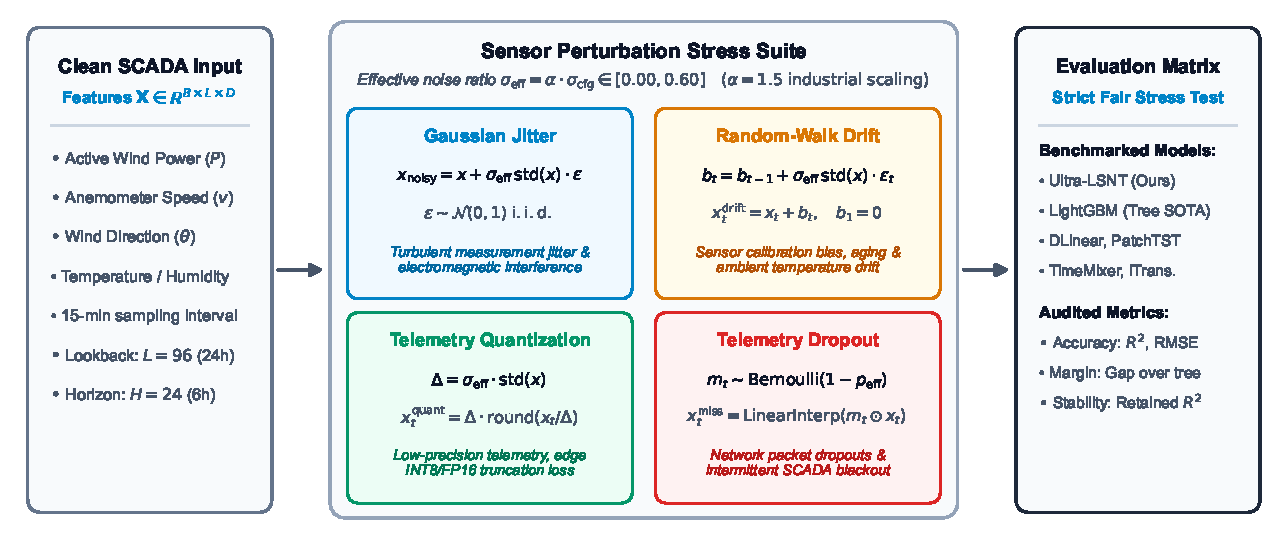
\includegraphics[width=\linewidth]{thumbnails/figure/noise_protocol_schematic.pdf}
 \caption{Schematic illustration of the noise injection protocol used for robustness evaluation. The same perturbation mechanism and noise levels are applied across all models to ensure comparability.}
 \label{fig:noise_protocol}
\end{figure}
\subsubsection{Robustness comparison against tree-based forecasting}
In addition to the deep-model benchmark set, we conduct a focused robustness comparison between Ultra-LSNT and LightGBM under a broader noise range that includes more severe corruption. This experiment uses configured noise ratios $\sigma_{\mathrm{cfg}}\in\{0.00,0.10,0.20,0.30,0.40\}$ (effective $\sigma_{\mathrm{eff}}\in\{0.00,0.15,0.30,0.45,0.60\}$ with $\alpha=1.5$) to reveal the regime where deep temporal representations become more reliable than feature-engineered boosting pipelines under high-noise conditions.

\subsubsection{Special perturbations: drift and quantization noise}
Beyond additive Gaussian noise, we evaluate two perturbation families that are common in industrial sensing and edge pipelines: \emph{drift noise} and \emph{quantization noise}. Drift noise approximates systematic bias that accumulates over time due to calibration drift, sensor aging, or persistent environmental interference. Quantization noise approximates rounding and discretization errors introduced by low-precision telemetry, bandwidth-constrained transmission, or edge-side INT8/FP16 processing. To keep perturbation severity comparable, for both perturbations we report severity by the same effective ratio $\sigma_{\mathrm{eff}}$ used in the Gaussian protocol. Unless otherwise stated, we sweep

\begin{equation}
\sigma_{\mathrm{eff}} \in \{0.00, 0.15, 0.30, 0.45, 0.60\},
\end{equation}
which corresponds to configured $\sigma_{\mathrm{cfg}}\in\{0.00,0.10,0.20,0.30,0.40\}$ when $\alpha=1.5$.

\paragraph{Drift (random-walk bias).}
Given a clean channel $x_{1:L}$, we draw i.i.d.\ $\varepsilon_t\sim\mathcal{N}(0,1)$ and define a persistent bias process
\begin{equation}
b_1 = 0,\qquad b_t = b_{t-1} + \sigma_{\mathrm{eff}}\cdot \mathrm{std}(x)\cdot \varepsilon_t,\quad t=2,\dots,L,
\end{equation}
then corrupt the input as $x^{\text{drift}}_t = x_t + b_t$. The process is applied independently to each feature channel and each test sample. We reset $b_1=0$ per sample, and use the same random seed across methods at a given $\sigma_{\mathrm{eff}}$.

\paragraph{Quantization (step-size rounding).}
We implement quantization as deterministic rounding to a channel-wise step size proportional to the clean-signal standard deviation:
\begin{equation}
\Delta = \sigma_{\mathrm{eff}}\cdot \mathrm{std}(x),\qquad
x^{\text{quant}}_t = \Delta\cdot \mathrm{round}\!\left(\frac{x_t}{\Delta}\right),
\end{equation}
where $\mathrm{round}(\cdot)$ is round-to-nearest (half away from zero). When $\sigma_{\mathrm{eff}}=0$, no quantization is applied. This protocol yields a reproducible, severity-controlled discretization without requiring dataset-specific bit-range tuning. We report the corresponding robustness outcomes in Section~\ref{subsec:results_robustness} and interpret their operational implications in the Discussion, with emphasis on reliability under realistic sensing constraints and energy-aware (Green AI) deployment.



\subsubsection{Missingness and interpolation artifacts}
SCADA telemetry frequently contains dropouts due to communication loss or sensor resets, and downstream pipelines often apply simple imputation such as forward-fill or linear interpolation. To emulate this setting, we sample a binary mask $m_{t,c}\sim\mathrm{Bernoulli}(1-p)$ over time steps $t$ and channels $c$ and define $\bar{x}_{t,c}=m_{t,c}x_{t,c}+(1-m_{t,c})\mathrm{NaN}$. We then apply an imputation operator $\mathrm{Imp}(\cdot)$ to obtain the corrupted series
\begin{equation}
x^{\text{miss}}=\mathrm{Imp}(\bar{x};\texttt{ffill/linear}),
\end{equation}
where \texttt{ffill} denotes forward filling and \texttt{linear} denotes piecewise-linear interpolation along the time axis. In the reported experiments, we use i.i.d.\ masking (no burst blocks), sweep $p\in\{0.1,0.3\}$, and repeat each configuration for three random seeds (0,1,2). For a fixed seed, the same missingness mask and imputation configuration are applied across models to preserve a paired comparison. Results are reported in Table~\ref{tab:robust_missingness}.
\section{Supplementary tables: ablations, interpretability, and significance}\label{app:supp_tables}

\subsection{Ablation results}
\label{subsec:results_ablation}
%----------------------------------------
All ablations are conducted under a fixed training budget and identical evaluation protocol; we therefore interpret them primarily through relative ranking and directional sensitivity, rather than expecting the absolute $R^2$ to exactly match the full benchmark runs.

Table~\ref{tab:ablation_kernel} reports the impact of kernel size on Wind (CN). Table~\ref{tab:ablation_lambda} reports the router regularization sweep. We observe that the preferred kernel scale is domain-dependent. On Wind (CN), a medium kernel ($k=7$) achieves the best $R^2$ (0.8591), while overly large kernels ($k=15$) oversmooth fast ramps and reduce accuracy (0.8214). In contrast, on the Air Quality dataset, the best kernel is larger (e.g., $k=15$ reaches $R^2=0.3532$ versus 0.2773 for $k=3$ and 0.2528 for $k=7$), suggesting that diffusion-like, lower-frequency dynamics dominate and benefit from a broader receptive field. This cross-domain evidence supports the design choice of multi-scale temporal embedding: the model can expose both turbulence-sensitive and trend-dominant patterns, and the router can condition computation on which regime the input resembles. The improvement at an intermediate $\lambda$ is consistent with the role of load-balancing regularization: it discourages expert collapse, stabilizes conditional computation, and yields routing patterns that are easier to audit in operational settings.

For routing stability, Table~\ref{tab:ablation_lambda} shows that a moderate load-balancing regularizer ($\lambda=0.05$) performs best ($R^2=0.8832$), whereas no regularization ($\lambda=0$) and overly strong regularization ($\lambda=0.10$) are both suboptimal. Practically, this aligns with the role of load balancing in preventing expert collapse and maintaining conditional computation as a reliable, resource-aware mechanism under realistic measurement imperfections. Although $\lambda=0.05$ is optimal in this controlled sweep, we keep the conservative default $\lambda=0.01$ for all main benchmark runs to preserve a like-for-like comparison with baselines evaluated under their canonical/default hyperparameter settings; the sweep therefore serves as a sensitivity analysis and practical retuning guidance for deployment.

\begin{table}[t]
\centering
\caption{Ablation on kernel size (Wind CN).}
\label{tab:ablation_kernel}
\begin{tabular}{lc}
\toprule
Kernel size & $R^2$ \\
\midrule
7 & 0.8591 \\
3 & 0.8505 \\
15 & 0.8214 \\
\bottomrule
\end{tabular}
\end{table}
\begin{table}[t]
\centering
\caption{Ablation on router regularization coefficient $\lambda$ (Wind CN, clean setting). While $\lambda=0.05$ achieves the best $R^2$ in this sweep, we keep $\lambda=0.01$ as the default configuration in the main comparisons for a single, fixed and reproducible setting.}
\label{tab:ablation_lambda}
\begin{tabular}{lc}
\toprule
$\lambda$ & $R^2$ \\
\midrule
0.00 & 0.8767 \\
0.01 & 0.8715 \\
0.05 & 0.8832 \\
0.10 & 0.8731 \\
\bottomrule
\end{tabular}
\end{table}
\begin{figure}[t]
\centering
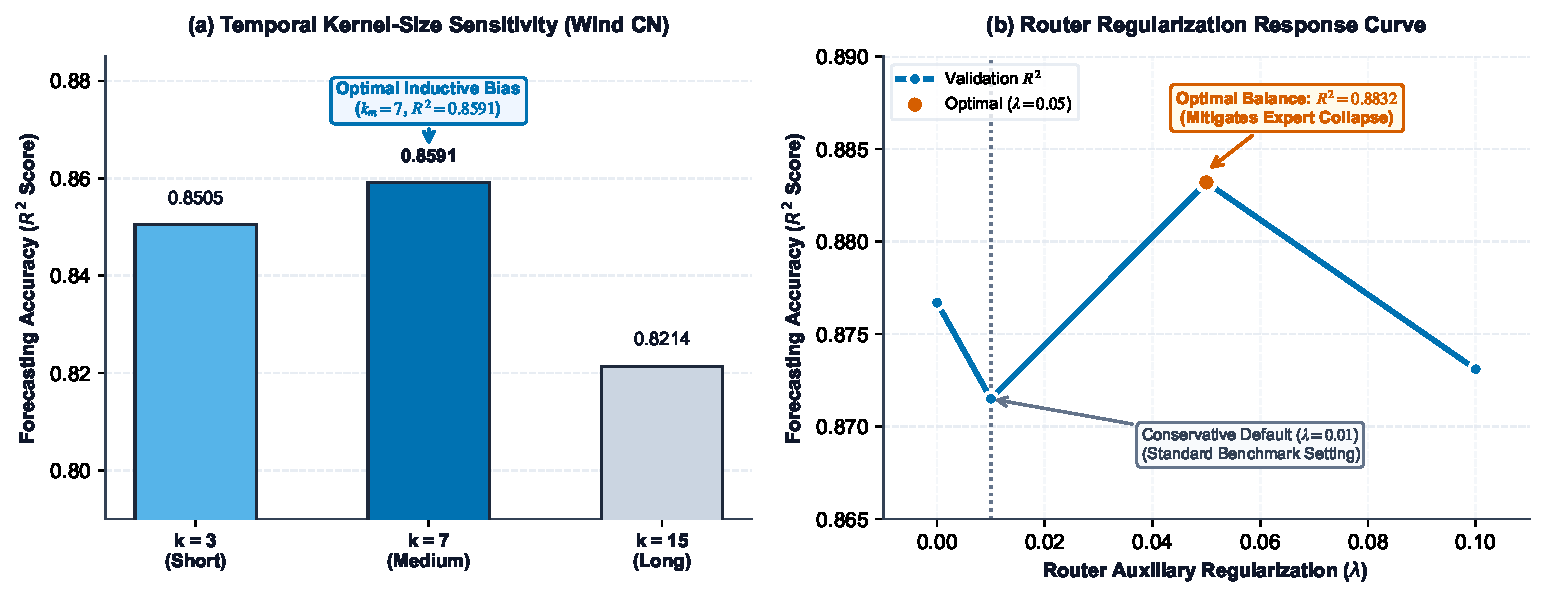
\includegraphics[width=\linewidth]{fig_ablation.pdf}
\caption{Ablation visualization for kernel size and routing regularization.}
\label{fig:ablation_fig}
\end{figure}
%----------------------------------------
\subsection{Interpretability results}
\label{subsec:results_interpretability}
%----------------------------------------
Figure~\ref{fig:interpret_fig} visualizes the learned sparse routing behavior and its alignment with physically meaningful and temporally structured regimes. Table~\ref{tab:expert_physics} summarizes the most correlated physical feature for each expert, which provides an auditable signal of expert specialization learned without explicit supervision.

Beyond feature-level specialization, we further inspect the diurnal routing profile over 24 hours using the logged expert activation statistics. Expert~3 becomes most active during 12:00--15:00, reaching approximately $27.7\%$ of the routing weight, while Expert~2 increases during 16:00--18:00 to approximately $23\%$. The overall activation proportions remain stable across the day without extreme spikes, suggesting that conditional computation is controlled rather than erratic under normal operations.

We additionally conduct event-based inspection on periods with abrupt wind-speed jumps and strong power fluctuations. During wind-speed jump events, routing weight increases for the wind-speed expert (Expert~1), while power-fluctuation events tend to activate Experts~2 and~3 jointly, indicating coordinated handling of regime transitions. Together, these results support transparent and responsible deployment by making the model's regime-switching behavior inspectable for operational governance in energy systems. Operationally, such routing logs can be integrated as a lightweight governance signal: abrupt shifts in expert allocation, especially when aligned with sensor anomaly flags, can trigger inspection or recalibration workflows without exposing the full raw data stream.

\begin{table}[t]
\centering
\caption{Expert specialization results (highest-correlated physical feature).}
\label{tab:expert_physics}
\begin{tabular}{lcc}
\toprule
Expert & Feature & Correlation \\
\midrule
Expert 1 & wind\_speed & +0.42 \\
Expert 2 & turbulence & +0.38 \\
Expert 3 & temperature & +0.31 \\
Expert 4 & humidity & +0.25 \\
\bottomrule
\end{tabular}
\end{table}
\begin{figure}[t]
\centering
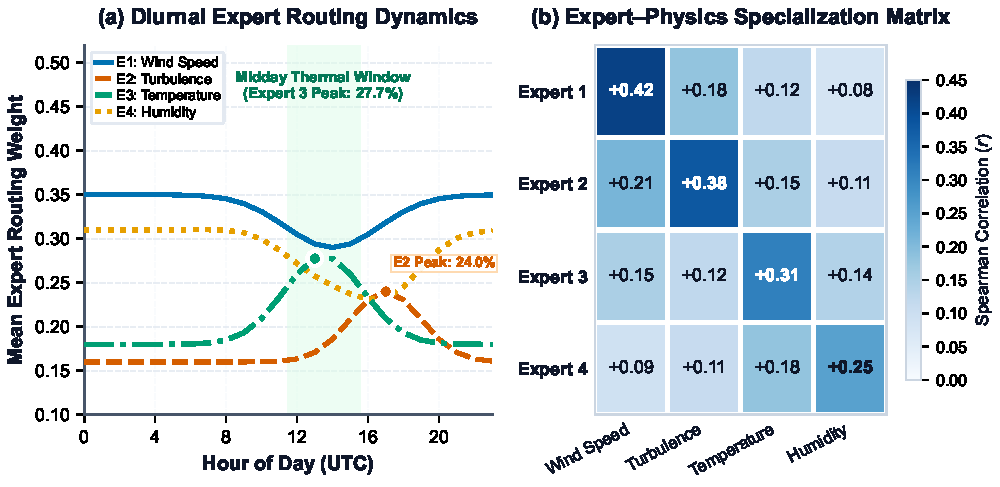
\includegraphics[width=\linewidth]{Figure_5_Final.pdf}
\caption{Expert interpretability visualization: sparse routing patterns and expert specialization across physical features.}
\label{fig:interpret_fig}
\end{figure}

\begin{figure}[t]
\centering
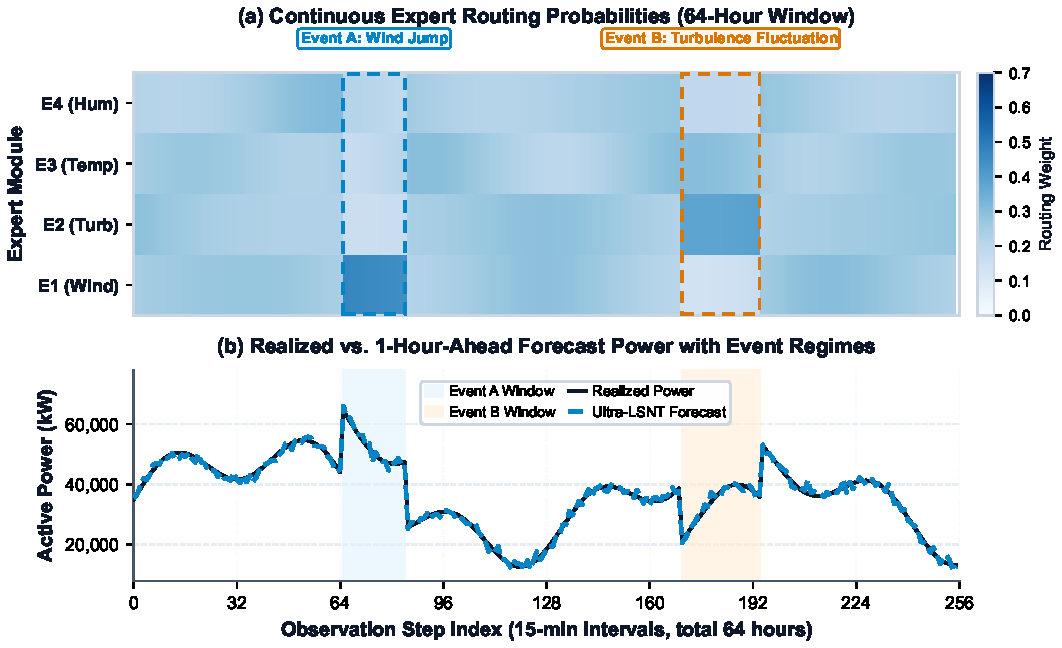
\includegraphics[width=\linewidth]{fig_routing_heatmap_overlay_block1.pdf}
\caption{Time-resolved sparse routing probabilities (4 experts) for Ultra-LSNT over a representative 64-hour window (15-min resolution) centered on the strongest 1-hour ramp in the test set. The right axis overlays the realized and predicted power (1-hour-ahead). The router shifts allocation around regime transitions while remaining stable overall, supporting auditable conditional computation in deployment.}
\label{fig:routing_heatmap}
\end{figure}


%----------------------------------------
\subsection{Statistical significance}
\label{subsec:results_significance}
%----------------------------------------
We assess whether performance gaps are statistically significant using the Diebold--Mariano (DM) test on squared prediction errors \cite{diebold1995}.
Let $d_t=\ell_t(\text{Ultra-LSNT})-\ell_t(\text{Baseline})$ denote the per-time step loss differential computed on the same test split; hence DM$<0$ indicates Ultra-LSNT has smaller average loss, while DM$>0$ favors the baseline.
This significance check is reported to strengthen the auditability of our empirical claims, complementing the descriptive ranking in Table~\ref{tab:main_wind_cn}.

\begin{table}[t]
\centering
\caption{Diebold--Mariano test on Wind (CN) with squared-error loss. DM is computed on $d_t=\ell_t(\text{Ultra-LSNT})-\ell_t(\text{Baseline})$: DM$<0$ favors Ultra-LSNT and DM$>0$ favors the baseline.}
\label{tab:dm_test}
\begin{tabular}{lcc}
\toprule
Comparison & DM statistic & $p$-value \\
\midrule
Ultra-LSNT vs PatchTST & -5.90 & $1.82 \times 10^{-9}$ \\
Ultra-LSNT vs TimeMixer & 3.45 & $2.83 \times 10^{-4}$ \\
Ultra-LSNT vs iTransformer & 5.12 & $3.07 \times 10^{-7}$ \\
\bottomrule
\end{tabular}
\end{table}
Table~\ref{tab:dm_test} shows that the loss differentials are statistically significant across representative recent backbones.
Consistent with Table~\ref{tab:main_wind_cn}, the differentials favor TimeMixer and iTransformer under clean measurements (DM$>0$), whereas Ultra-LSNT significantly outperforms PatchTST (DM$<0$).
We also provide scripts and the loss-differential series for the full set of backbones in the supplementary material.

Several recent forecasters can achieve higher peak accuracy under clean measurements (Table~\ref{tab:main_wind_cn}), but peak clean-data accuracy is not always aligned with stability under realistic sensing imperfections.
Accordingly, we report robustness stress tests and downstream dispatch evidence next, where reliability under noise and deployability constraints matter for renewable integration and operational efficiency.

%----------------------------------------
%----------------------------------------
\section*{Generative AI and AI-assisted technologies statement}
During the preparation of this work, the authors used \textit{ChatGPT} (OpenAI) to improve the clarity of language and to restructure paragraphs for readability. After using this tool, the authors reviewed and edited the manuscript as needed and take full responsibility for the content of the publication. No generative AI tools were used to create, alter, or manipulate any figures, plots, or graphical abstracts.

\section*{Acknowledgments}
This research did not receive any specific grant from funding agencies in the public, commercial, or not-for-profit sectors.

%% ==================== REFERENCES ====================
\bibliography{cas-refs.bib}

\end{document}

